\documentclass[shortpres]{beamer}
\usetheme{CambridgeUS}
\usepackage[utf8]{inputenc}
\usepackage[style=authortitle,backend=bibtex]{biblatex}
\addbibresource{references.bib}
\usepackage{fnpct}
\AdaptNoteOpt\footcite\multfootcite
\renewcommand{\footnotesize}{\tiny}
\renewcommand*{\bibfont}{\small
}
\setbeamertemplate{footline}
{
  \leavevmode%
  \hbox{%
  \begin{beamercolorbox}[wd=.333333\paperwidth,ht=2.25ex,dp=1ex,center]{author in head/foot}%
    \usebeamerfont{author in head/foot}\insertshortauthor%~~						\beamer@ifempty{\insertshortinstitute}{}{(\insertshortinstitute)}
  \end{beamercolorbox}%
  \begin{beamercolorbox}[wd=.333333\paperwidth,ht=2.25ex,dp=1ex,center]{title in head/foot}%
    \usebeamerfont{title in head/foot}\insertshorttitle
  \end{beamercolorbox}%
  \begin{beamercolorbox}[wd=.333333\paperwidth,ht=2.25ex,dp=1ex,right]{date in head/foot}%
    \usebeamerfont{date in head/foot}\insertshortdate{}\hspace*{2em}
    \insertframenumber{} / \inserttotalframenumber\hspace*{2ex}
  \end{beamercolorbox}}%
  \vskip0pt%
}\part{title}
\beamertemplatenavigationsymbolsempty


%color specification---------------------------------------------------------------
\definecolor{TUMblue}{rgb}{0.00, 0.40, 0.74}
\definecolor{TUMgray}{rgb}{0.85, 0.85, 0.86}
\definecolor{TUMpantone285C}{rgb}{0.00, 0.45, 0.81}
\definecolor{lightblue}{rgb}{0.7529,0.8118,0.9333}

\setbeamercolor{block title}{fg=white, bg=TUMpantone285C}
\setbeamercolor{block body}{bg=lightblue}
\setbeamertemplate{blocks}[rounded][shadow=true]
%----------------------------------------------------------------------------------

\setbeamercolor{frametitle}{fg=TUMblue, bg=white}
\setbeamercolor{palette primary}{fg=TUMblue,bg=TUMgray}
\setbeamercolor{palette secondary}{use=palette primary,fg=TUMblue,bg=white}
\setbeamercolor{palette tertiary}{use=palette primary,fg=white, bg=TUMblue}
\setbeamercolor{palette quaternary}{use=palette primary,fg=white,bg=TUMpantone285C}


\setbeamercolor{title}{bg=white,fg=TUMblue}
\setbeamercolor{item projected}{use=item,fg=black,bg = lightblue}
\setbeamercolor{block title}{fg=black, bg=lightblue}
\setbeamercolor{block body}{bg=white}
\setbeamertemplate{blocks}[rounded][shadow=true]
%----------------------------------------------------------------------------------
\setcounter{figure}{0}


\usepackage{psfrag} %for \psfrag in figures
\usepackage{algorithm,algpseudocode}  %for algorithm environment
\usepackage{graphicx}

\title[Motion Planning for Autonomous Vehicles]{Clustering Similar Traffic Scenarios}

\author[\"Uste, Chen, Liu, Ramneantu]{Murat Can \"Uste, Zhaoying Chen, Qiaoxi Liu, Emanuel Ramneantu}
\institute[TU M\"unchen]{Technische Universit\"at M\"unchen}

\date{Feb 3, 2020}

\begin{document}

\begin{frame}
    \titlepage
\end{frame}

\section{Problem Statement}	

\begin{frame}{Problem of Testing Automated Vehicle Functions}	

\begin{itemize} 
\item How do we test automated vehicle functions?
\vfill \item  Can we cover all situations that occur in a traffic?
\vfill \item  Do we know all different situations that can occur, especially in microscopic level?
\end{itemize}
\end{frame}

\section{Proposed Method}	

\begin{frame}{Proposed Method}	

\begin{itemize} 
\item \textbf{Cluster similar scenarios} in order to group them based on their similarity, and test automated vehicle functions on a set of scenarios from each group to reduce testing and validation effort.
\end{itemize}

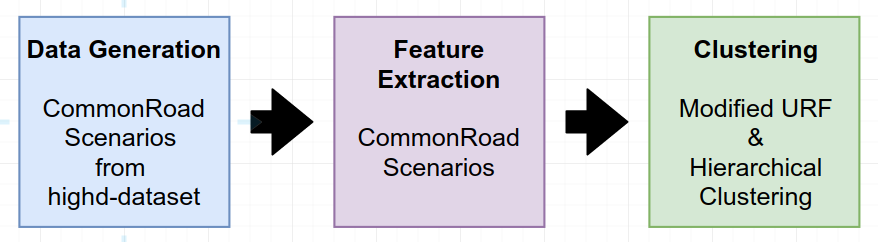
\includegraphics[width=\textwidth]{proposed_01}
\end{frame}

\section{Tasks}	

\begin{frame}{Tasks}	

\begin{itemize} 
\item Data generation
\vfill \item Feature extraction
\vfill \item Unsupervised Random Forest and Hierarchical Clustering
\end{itemize}
\end{frame}

\section{Data Generation}	

\begin{frame}{HighD Dataset}	

\begin{figure}[h!]
  \centering
  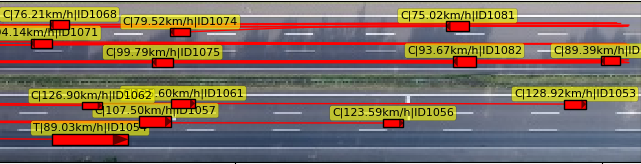
\includegraphics[width=\textwidth]{highd-example}
  \vspace{-2em}
  \caption{Visualization of the a recording using the tools provided.}
\end{figure}

\begin{itemize} 
\item 60 recordings from 6 different highway locations in Germany with different traffic states (e.g. traffic jams).
\vfill \item 110.500 vehicles, 147 driven hours.
\vfill \item \textbf{Pre-extracted Information:} vehicle types, sizes, trajectories, and metrics such as THW and TTC, as well as lane changes. 
\vfill \item Road length is 420 meters, and positioning error is below 10cm.
\end{itemize}

\end{frame}


\section{Data Generation}	

\begin{frame}{HighD to CommonRoad Scenarios}	

\begin{itemize} 
\item Extract 3.24 sec. segments from raw data and convert them to CommonRoad Scenario format. It results in 81 time steps with dt=0.04, since the fps of recordings are 25.
\vfill \item \textbf{Don't convert segments that pose no challange in terms of motion planning (e.g. free driving scenarios)}.
	\begin{itemize} 
	\item Based on Min DHW, Min THW, and Min TTC of tracks, and lane change information.
	\end{itemize}
\vfill \item Select a frame from recording based on criticality and set it as the middle time step of the extracted segment.
	\begin{itemize} 
	\item Example: Select 1000th frame of recording (40th second) as the middle frame, and extract the segment between 960th and 1040th frames.
	\end{itemize}
\end{itemize}

%\vfill 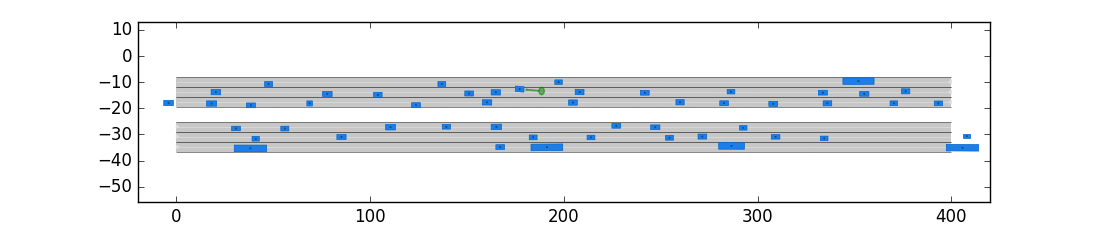
\includegraphics[width=\textwidth]{cr-example-15}

\end{frame}

\section{Data Generation - DHW, THW, and TTC}	

\begin{frame}{DHW, THW, and TTC}	

\begin{center}
    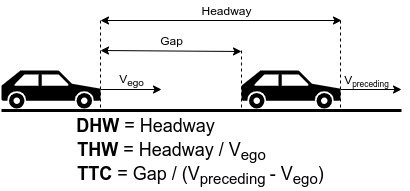
\includegraphics[width=7cm]{dhw_thw_ttc}
\end{center}

\begin{itemize} 
\fontsize{9pt}{10pt}\selectfont \item \textbf{Distance Headway (DHW):} Distance between the front of the ego vehicle and the front of the preceding obstacle in the same lane.
\fontsize{9pt}{10pt}\selectfont \item \textbf{Time Headway (THW):} The time required for the ego vehicle's front to reach same position as the preceding obstacle's front, if it continues with its current speed.
\fontsize{9pt}{10pt}\selectfont \item \textbf{Time to Collision (TTC):} The time required for there to be a collision between the ego vehicle and the preceding vehicle, if they continue with their current speed.
\end{itemize}

\end{frame}

\section{Data Generation - Filtering Critical Scenarios}	

\begin{frame}{Filtering Critical Scenarios}	

\begin{itemize} 
\fontsize{9pt}{10pt}\selectfont \item Critical maneuvers detected on the dataset \footcite{highDdataset}\footcite{benmimoun2011incident}:
	\begin{itemize} 
	\fontsize{9pt}{10pt}\selectfont \item \textbf{Free Driving (Longitudinal uninfluenced driving):} Driving without being influenced by a preceding vehicle.
	\fontsize{9pt}{10pt}\selectfont \item \textbf{Vehicle Following (Longitudinal influenced driving):} Actively following another vehicle.
	\fontsize{9pt}{10pt}\selectfont \item \textbf{Critical Maneuver:} Low TTC or THW to a preceding vehicle
	\fontsize{9pt}{10pt}\selectfont \item \textbf{Lane Change:} Crossing lane markings and staying on a new lane 
	\end{itemize}	
\end{itemize}

\begin{center}
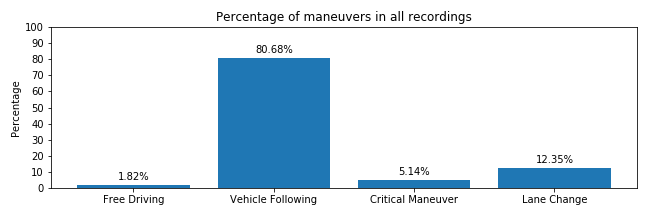
\includegraphics[width=11cm]{raw_maneuvers}
\end{center}

\end{frame}

\section{Data Generation - Filtering Process}	

\begin{frame}{Filtering Process}	

Following steps are performend on \textbf{each recording} to filter out critical frames of the recording based on lane change information and one of the DHW, THW, or TTC metrics of each track.\\

\begin{itemize} 
\item \textbf{Step 1:} Filter out tracks that don't have the selected metric defined.
\item \textbf{Step 2:} Filter out tracks that don't perform lane change maneuver if we want to use only the lane changing tracks for frame selection, otherwise don't filter.
\item \textbf{Step 3:} Sort each track's frames based on selected metric, and select the frame with minimum value for each track.
\item \textbf{Step 4:} Generate scenarios by setting the selected frames as the middle time step.
\end{itemize}

\end{frame}

\section{Data Generation - Scenario Generation Process}	

\begin{frame}{Scenario Generation Process}	

Following steps are performed on \textbf{each filtered frame} on \textbf{each recording} after the critical frames with their associated tracks have been filtered.\\

\begin{itemize} 
\item \textbf{Step 1:} Discard if there are not enough time steps for the selected track when the associated frame is selected as the middle time step.
\item \textbf{Step 2:} Discard if the initial position or final position is too close to the scenario's edges (in order to have meaningful features during the feature extraction process).
\item \textbf{Step 3:} Discard lanelets and tracks that are in the opposite direction (physically seperated, have no effect on the scenario).
\item \textbf{Step 4:} Generate dynamic obstacles from all vehicles within the selected initial and final time frames.
\item \textbf{Step 5:} Set the id of the dynamic obstacle of the selected frame's track to ego vehicle's id (99 in our case).
\end{itemize}

\end{frame}

\section{Data Generation - Scenario Examples}	

\begin{frame}{Scenario Examples}
\begin{itemize}
	\item Visualization of a scenario where ego vehicle follows the preceding vehicle.
\end{itemize}
\begin{figure}[h!]
  \centering
  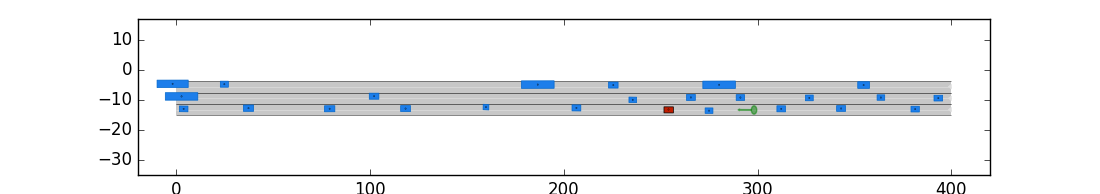
\includegraphics[width=\textwidth]{MPP_DEU_LocationA-11_T880F7378_T-1}
\end{figure}
\begin{itemize}
	\item Visualization of a scenario where ego vehicle changes lanes.
\end{itemize}
\begin{figure}[h!]
  \centering
  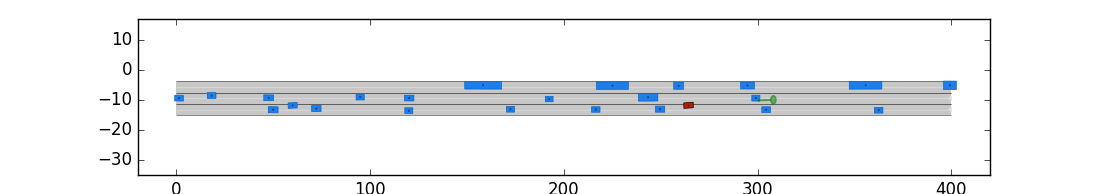
\includegraphics[width=\textwidth]{MPP_DEU_LocationA-11_T1164F9870_T-1}
\end{figure}
\end{frame}

\section{Data Generation - Generated Datasets}	

\begin{frame}{Generated Datasets}	

\begin{tabular}{ |p{2.3cm}||p{2.5cm}|p{3.2cm}|p{2cm}|  }
 \hline
 \multicolumn{4}{|c|}{CommonRoad Scenario Datasets} \\
 \hline
 Dataset Name & Selected Metric & Only Lane Changing & Sample Size\\
 \hline
 DHW Small & Min DHW & True  & 6.551\\
 THW Small & Min THW & True  & 6.544\\
 TTC Small & Min TTC & True  & 6.944\\
 DHW Big   & Min DHW & False & 44.812\\
 THW Big   & Min THW & False & 44.107\\
 TTC Big   & Min TTC & False & 44.280\\
 \hline
\end{tabular}

\vfill

\begin{itemize} 
\item Scenario names are in the following format:\\
\fontsize{8pt}{15pt}\selectfont\texttt{MPP\_DEU\_<location id>-<recording id>\_T<ego track id>F<selected frame>\_T-1}
	\begin{itemize} 
	\fontsize{7pt}{10pt}\selectfont\item \textbf{location id:} One of the six recording locations
	\fontsize{7pt}{10pt}\selectfont\item \textbf{recording id:} Id of the recording
	\fontsize{7pt}{10pt}\selectfont\item \textbf{ego track id:} Track ID of the ego vehicle from the raw dataset.
	\fontsize{7pt}{10pt}\selectfont\item \textbf{selected frame:} Selected frame from the recording
	\end{itemize}
\end{itemize}

\end{frame}

\section{Data Generation - Maneuver Statistics}	

\begin{frame}{Maneuver Statistics on Generated Datasets}	

\begin{center}
	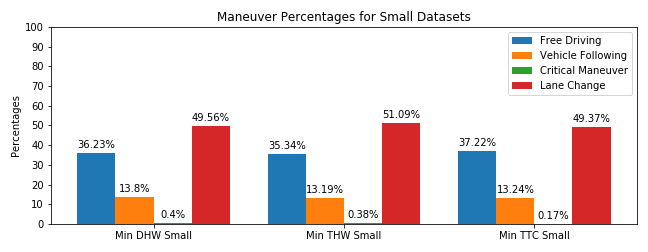
\includegraphics[width=12cm]{small_datasets_maneuvers}
\end{center}

\begin{itemize} 
\fontsize{8pt}{10pt}\selectfont\item The ratio of Free Driving maneuvers are higher compared to the raw dataset, because we limit the distance to 100 meters in order to simulate sensor range.
	\begin{itemize} 
		\fontsize{8pt}{10pt}\selectfont\item Some part of the Vehicle Following maneuvers are now considered Free Driving, because the preceding obstacle is further than 100 meters.
		\fontsize{8pt}{10pt}\selectfont\item Same case is also true for the Lane Change Maneuvers.
	\end{itemize}
\end{itemize}

\end{frame}

\section{Data Generation - Maneuver Statistics}	

\begin{frame}{Maneuver Statistics on Generated Datasets}	

\begin{center}
	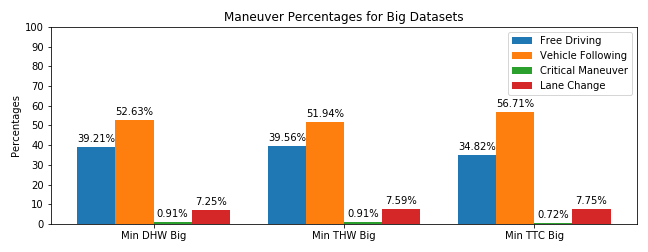
\includegraphics[width=12cm]{big_datasets_maneuvers}
\end{center}

\begin{itemize}
\fontsize{8pt}{10pt}\selectfont\item The ratio of critical maneuvers are also significantly lower compared to the raw dataset, because they calculate the DHW and other metrics based on the edge of the map as well.
	\begin{itemize} 
		\fontsize{8pt}{10pt}\selectfont\item They are either filtered out during the scenario generation process, or considered as Free Driving maneuver (since the minimum of DHW or other metrics are selected after sorting).
	\end{itemize}
\end{itemize}

\end{frame}


\section{Feature Extraction}	

\begin{frame}{Feature Extraction}	

\begin{itemize} 
\item How to build a quantitative model for the scenario
\vfill \item The goal of feature extraction: to give an approximate balance to capture the characteristics of scenarios, while being compact for fast computation
\vfill \item Model
\vfill \item Example
\vfill \item How to select crucial features
\end{itemize}
\end{frame}

\section{Feature Extraction}

\begin{frame}{Scenario Model}
    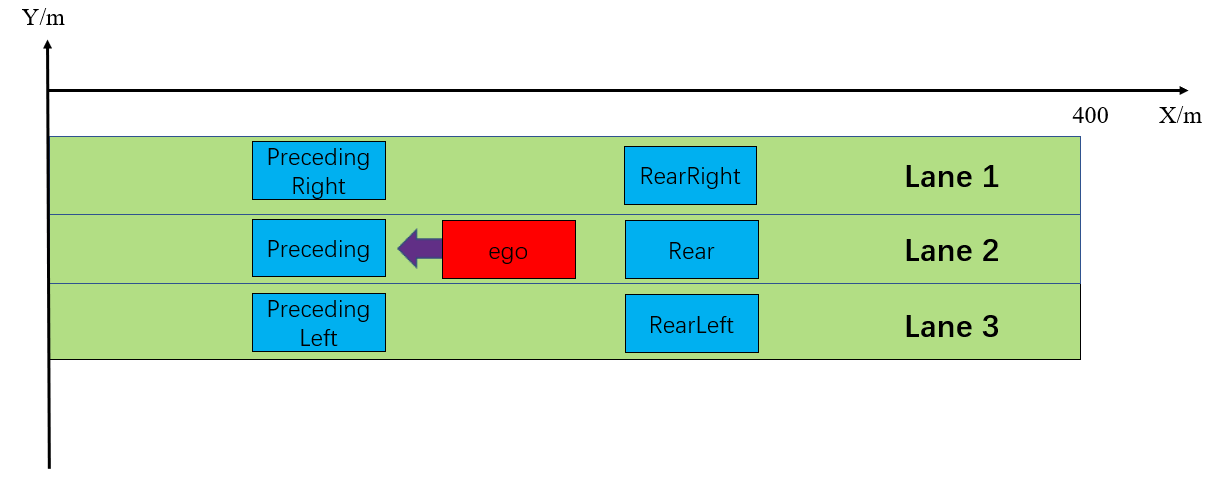
\includegraphics[height=0.6\textheight]{fig_FeatureExtraction/ScenarioModel.png}
\end{frame}

\section{Feature Extraction}

\begin{frame}{Previous Feature Structure}
    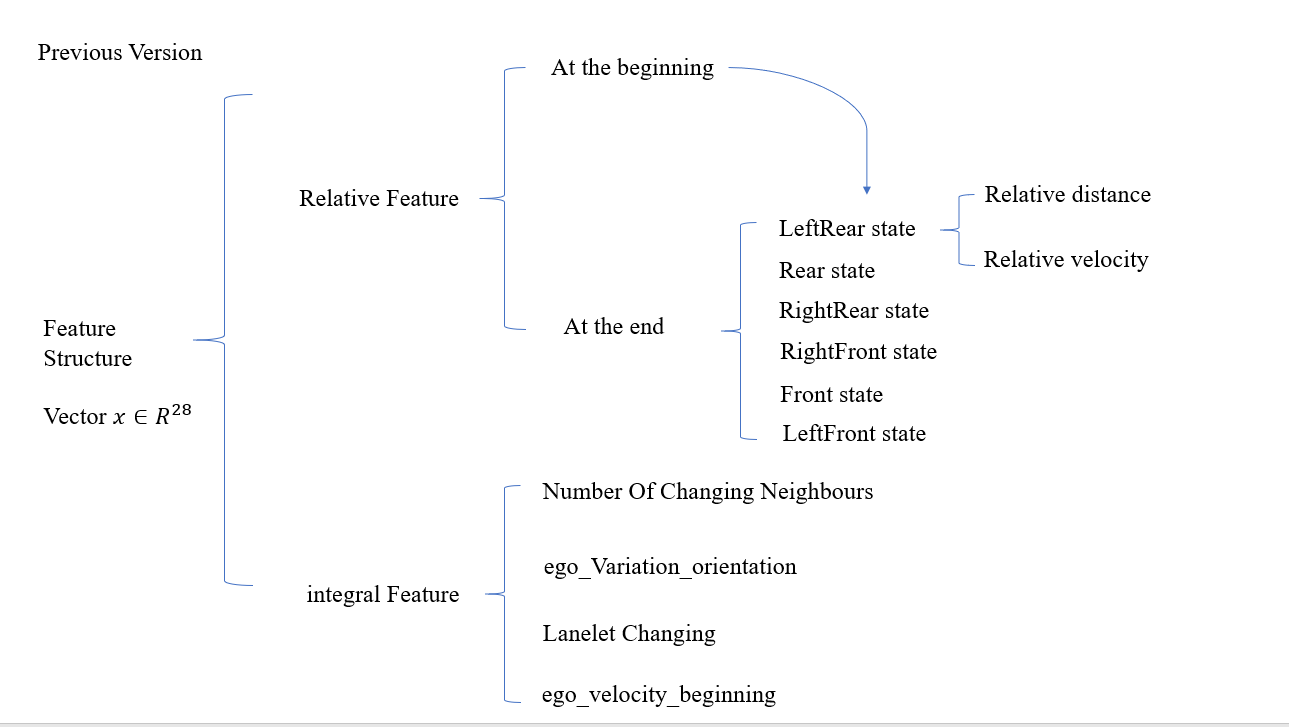
\includegraphics[width=12cm,height=6.5cm]{fig_FeatureExtraction/PreviousVersion.png}
\end{frame}

\section{Feature Extraction}

\begin{frame}{Current Feature Structure}
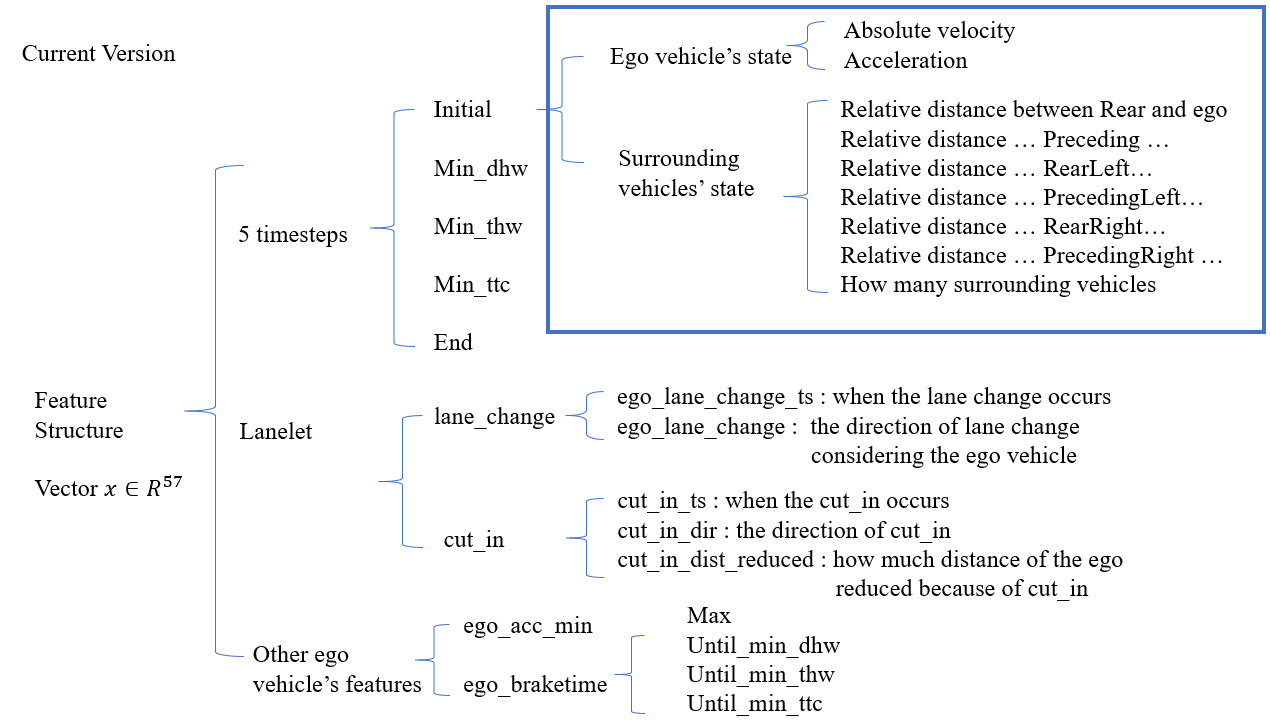
\includegraphics[height=0.6\textheight]{fig_FeatureExtraction/CurrentVersion.png}
\end{frame}



\section{Feature Extraction}
\begin{frame}{Compare}
\begin{itemize} 
	\item (1) Consider more time steps—which are more informative
	\vfill \item (2) Calculate more complex features like brake time, acceleration and cut in features
\end{itemize}
\end{frame}

\section{Feature Extraction}
\begin{frame}{Example}
	\textbf{Example:} MPP-DEU-LocationA-11-T1220F10351-T-1-40
    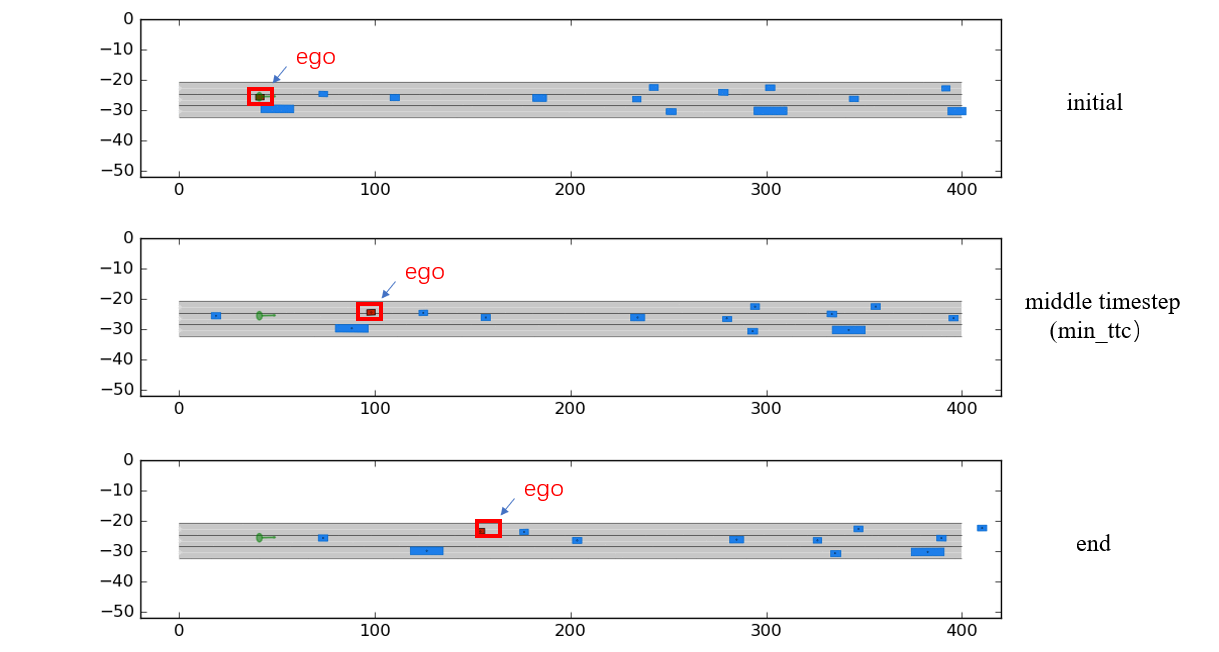
\includegraphics[width=12cm,height=6cm]{fig_FeatureExtraction/example.png}
\end{frame}

\section{Feature Extraction}
\begin{frame}{Example}
	\textbf{Example:} MPP-DEU-LocationA-11-T1220F10351-T-1-40
    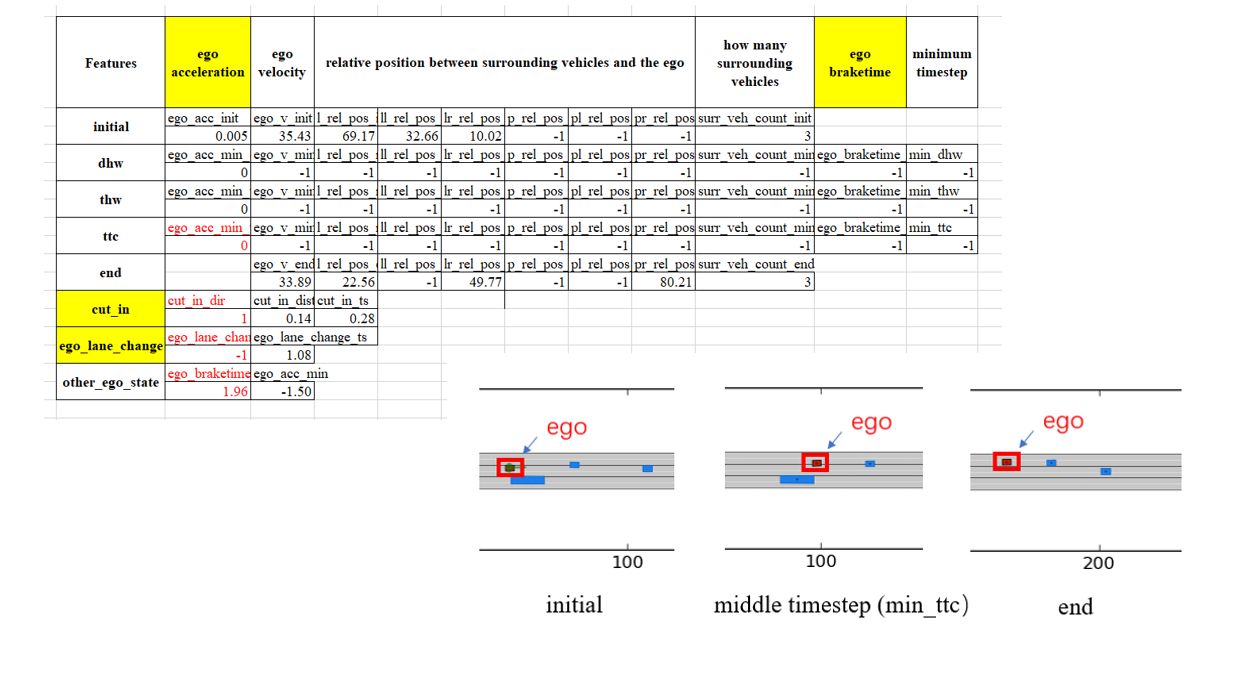
\includegraphics[height=0.75\textheight]{fig_FeatureExtraction/CrucialFeatureExplanation.png}
\end{frame}

\section{Feature Extraction}
\begin{frame}{How to select crucial features}
\textbf{What is crucial: }
\begin{itemize} 
	\item Intuitively: the more complex features contain more information
	
	\vfill \item Statistically\\
	(1) ego lane change > brake time > acceleration > how many surrounding vehicles > cut in\\
	(2) ego vehicle’s state > surrounding vehicles’ state
\end{itemize}
\begin{figure}
	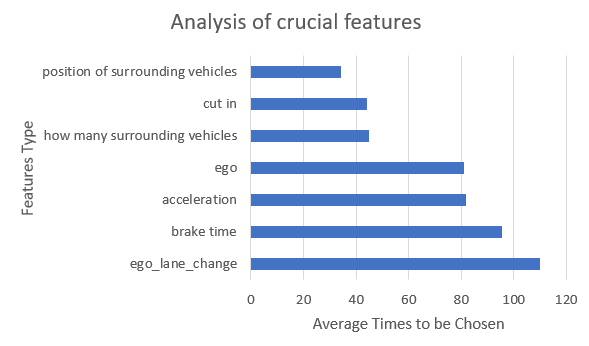
\includegraphics[height=0.5\textheight]{fig_FeatureExtraction/analysis_crucial_features.png} 
\end{figure}
\end{frame}

\section{Feature Extraction}
\begin{frame}{How to select crucial features}
	Statistical data for 300 trees of dataset: dhw-only-lanechanging dataset\\max depth of tree = 5
	\begin{figure}
			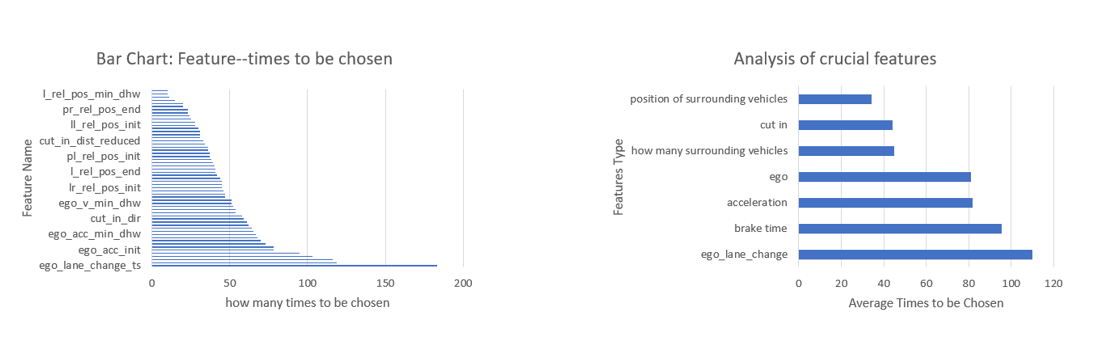
\includegraphics[height=0.45\textheight]{fig_FeatureExtraction/StatisticallyAnalysis.png} 
	\end{figure}
\end{frame}


\section{Clustering}	

\begin{frame}{Clustering}	
\begin{itemize} 
\item Motivation and Introduction of Random Forest (RF)
\vfill\item Challenges of RF
\vfill\item Implementation of RF and Proximity Matrix
\end{itemize}
\end{frame}
\begin{frame}{Motivation choosing Rondam Forest (RF)}	
  Our dataset:
  \begin{itemize} 
    \item High dimensional
    \item Value varies widely (also include missing values)
 \end{itemize}
  \begin{block}{We want...}
    model to be simple and explainable;
    \end{block}
    \begin{block}{We don't want...}
    to worry about feature selection or regularization.
      \end{block}
   Thus, the probable answer is Random Forest!
  
\end{frame}
\begin{frame}{Decision Tree (DT) to Random Forest (RF)}	
  taking subset \textbf{and} features randomly to build multiple DT.\\
  \begin{figure}
    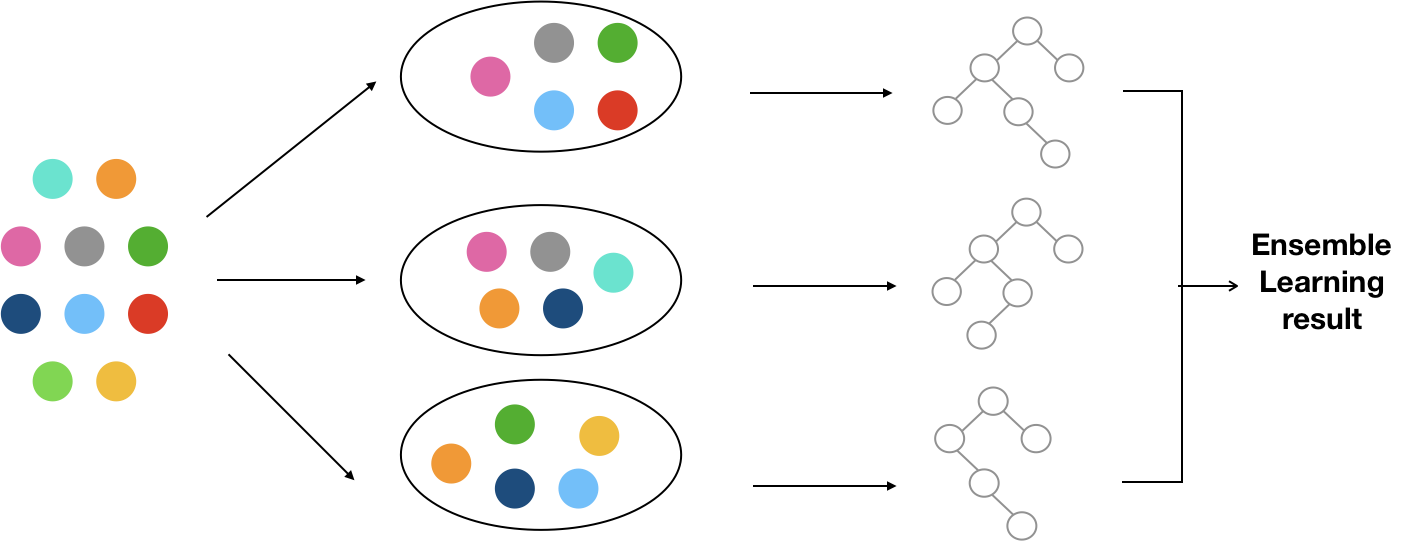
\includegraphics[height=0.5\textheight]{fig/bagging.png} 
  \end{figure}
\begin{itemize} 
  \item Can handle categorical/numerical features. Very little pre-processing. 
  \item Accuracy for missing data/outliers
  \item Quick training in terms of using subset and square root of features
\end{itemize}

\end{frame}
\begin{frame}{Challenge 1 How to apply RF as unsupervised method?}	
  \textbf{With labels} With labels, easily to get and evaluate result in terms of feature's value
  \begin{figure}
    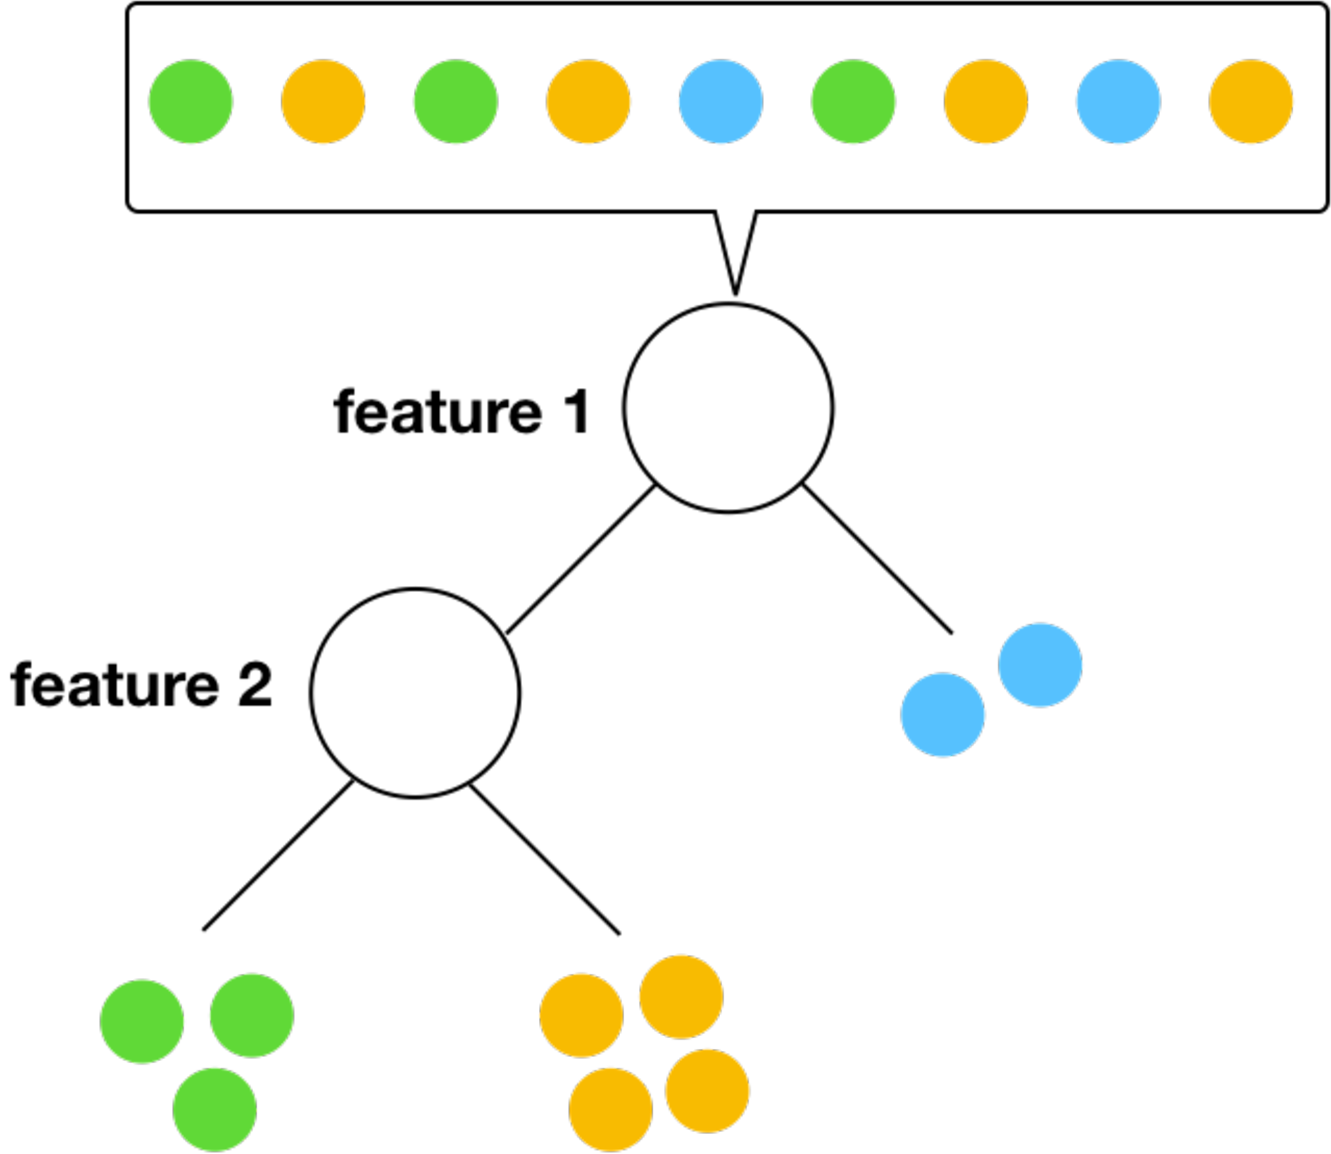
\includegraphics[height=0.6\textheight]{fig/normalrf.pdf} 
  \end{figure}
\end{frame}

  \begin{frame}{Challenge 1 Solution}	
    \textbf{Without labels...!} 
    \begin{itemize} 
      \item Adding same label (e.g. 0) for orginial data $(\mathcal{D})$ and generate synthetic data $(\mathcal{S})$ labeled with 1
      \item Training them together as normal DT
    \end{itemize}
      \begin{figure}
        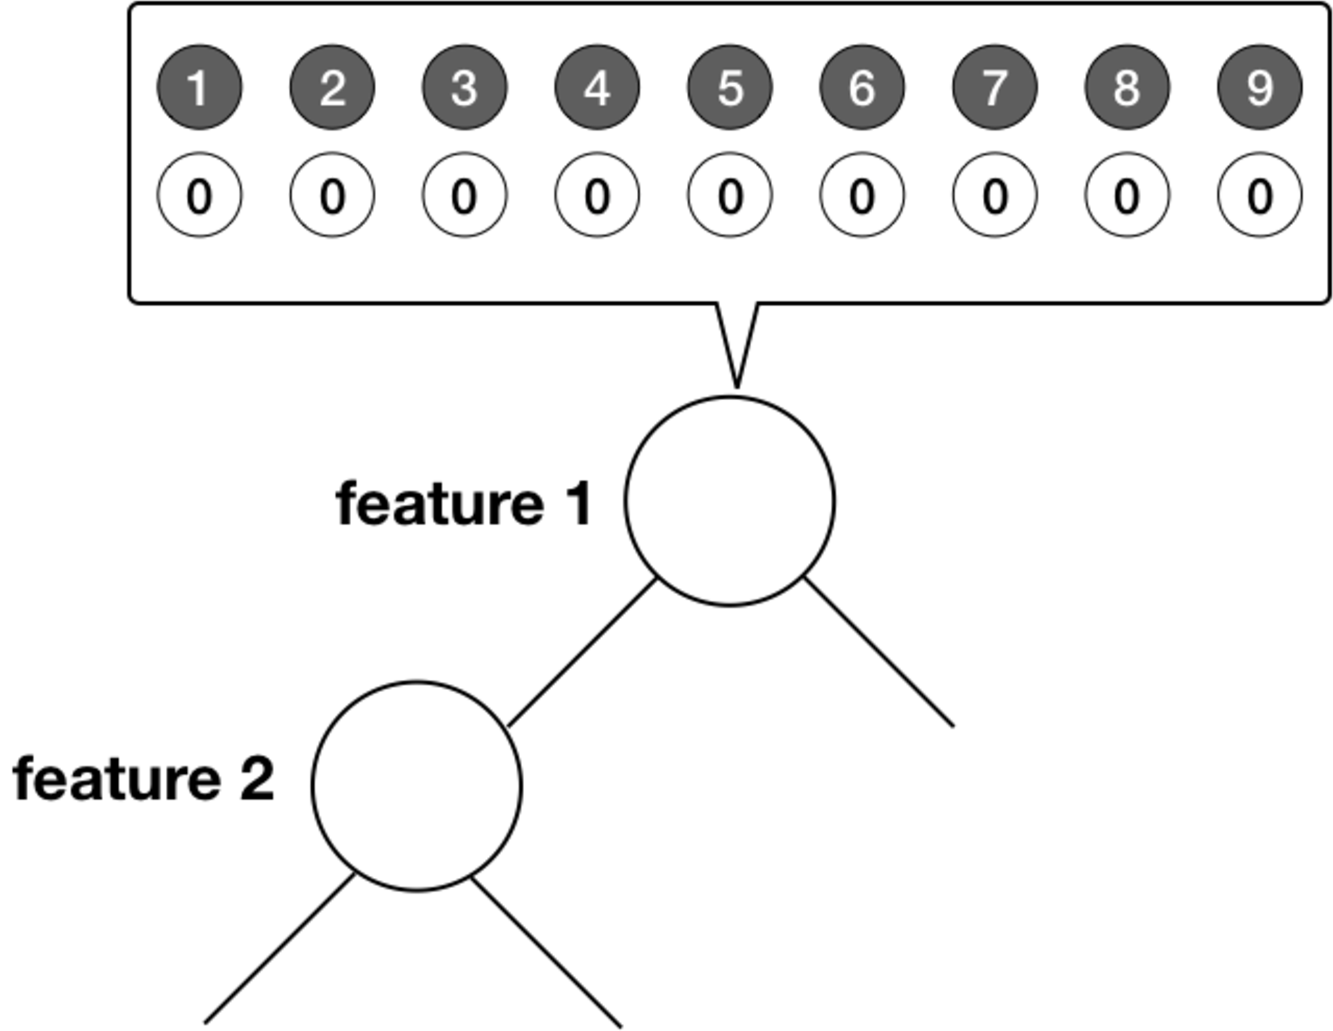
\includegraphics[height=0.5\textheight]{fig/noiserf.pdf} 
      \end{figure}
      \end{frame}
      \begin{frame}{Split Demo}
        \begin{figure}
          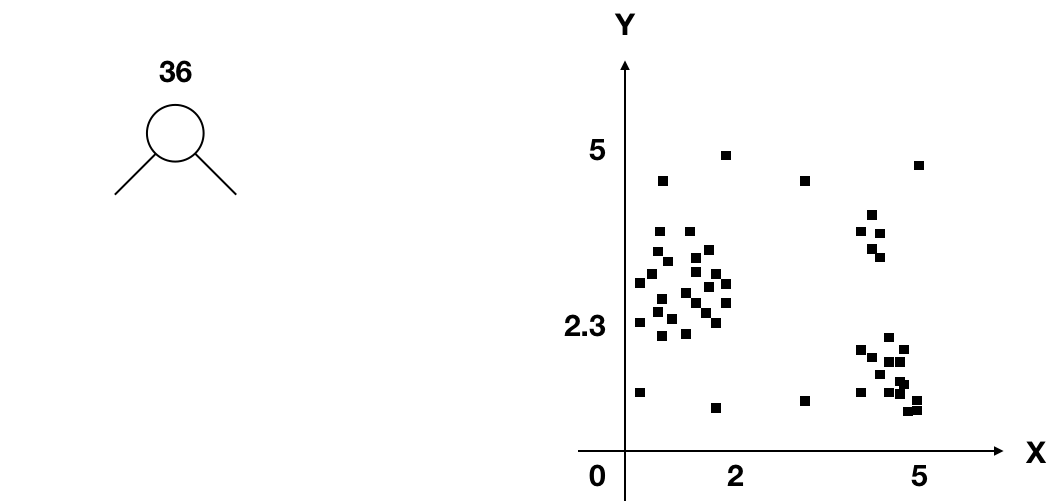
\includegraphics[height=0.65\textheight]{fig/split00}
        \end{figure}
      \end{frame}
      \begin{frame}{Split Demo}
          \begin{figure}
            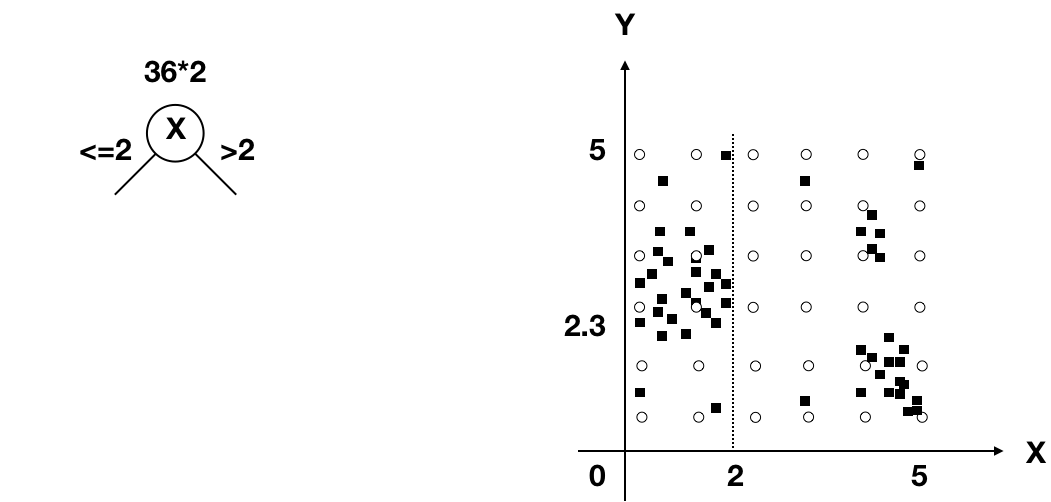
\includegraphics[height=0.65\textheight]{fig/split0}
          \end{figure}
        \end{frame}
        \begin{frame}{Split Demo}
          \begin{figure}
            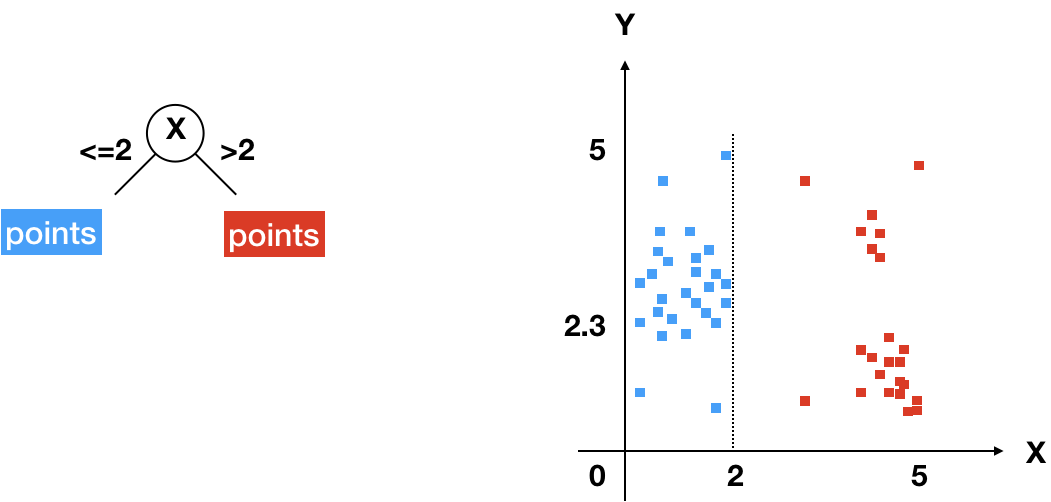
\includegraphics[height=0.65\textheight]{fig/split1}
          \end{figure}
        \end{frame}
        \begin{frame}{Split Demo}
          \begin{figure}
            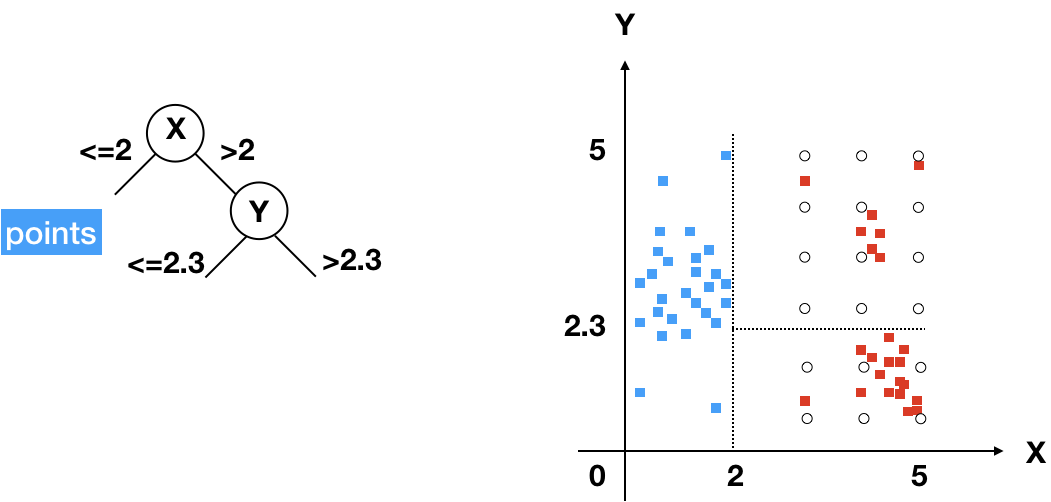
\includegraphics[height=0.65\textheight]{fig/split2}
          \end{figure}
        \end{frame}
        \begin{frame}{Split Demo}
          \begin{figure}
            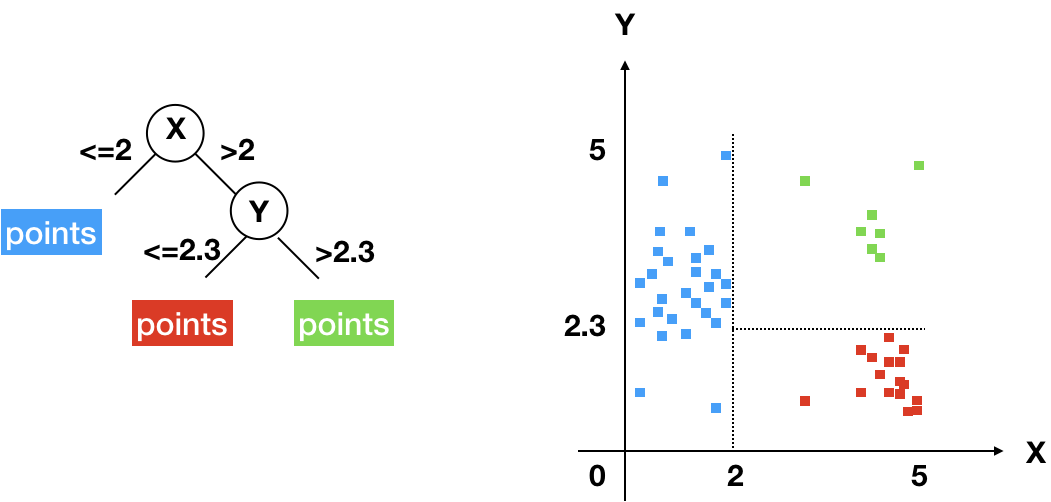
\includegraphics[height=0.65\textheight]{fig/split3}
          \end{figure}
        \end{frame}
  
  \begin{frame}{Challenge 2 How to measure similarity?}	
    The path of scenario i (as a part of one leaf) defined as $P_i$.\\
    $P_i$ = 0\textbf{L}1\textbf{R}2\textbf{L}
    \begin{figure}
      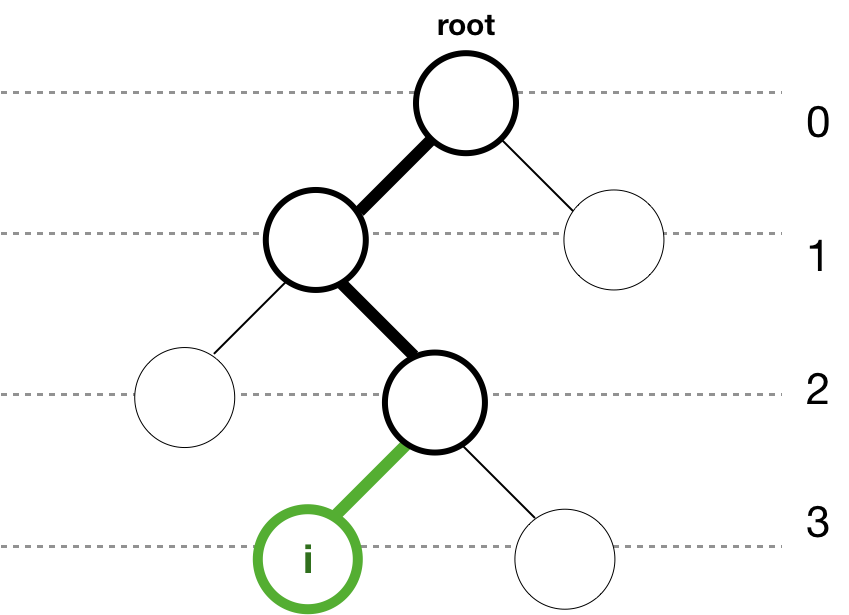
\includegraphics[height=0.6\textheight]{fig/ppath.png}
    \end{figure}
  \end{frame}
  \begin{frame}{Challenge 2 Solution: Proximity Path}
    $P_i$ = 0\textbf{L}1\textbf{R}2\textbf{L}\\
    $P_j$ = 0\textbf{L}1\textbf{R}2\textbf{R}\\
    Intersection: $|P_i \cap P_j| = 3$ \\
    Union: $|P_i|+ |P_j|-|P_i \cap P_j| = 4+4-3 = 5$
    \begin{figure}
      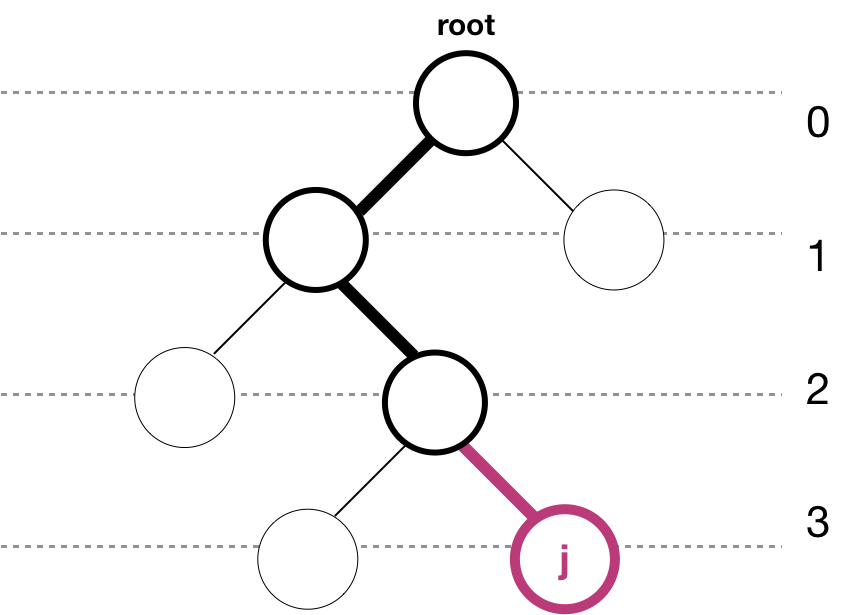
\includegraphics[height=0.6\textheight]{fig/ppath2.png}
    \end{figure}
  \end{frame}

  \begin{frame}{Proximity Path}	
  the Proximity (Jaccard Index) between i,j is:
  $$P_{ij}=\frac{|P_i \cap P_j|}{|P_i \cup P_j|} = \frac{3}{5}\in (0,1]$$ 0: no mutual path; 1: exactly same path
    \begin{figure}
      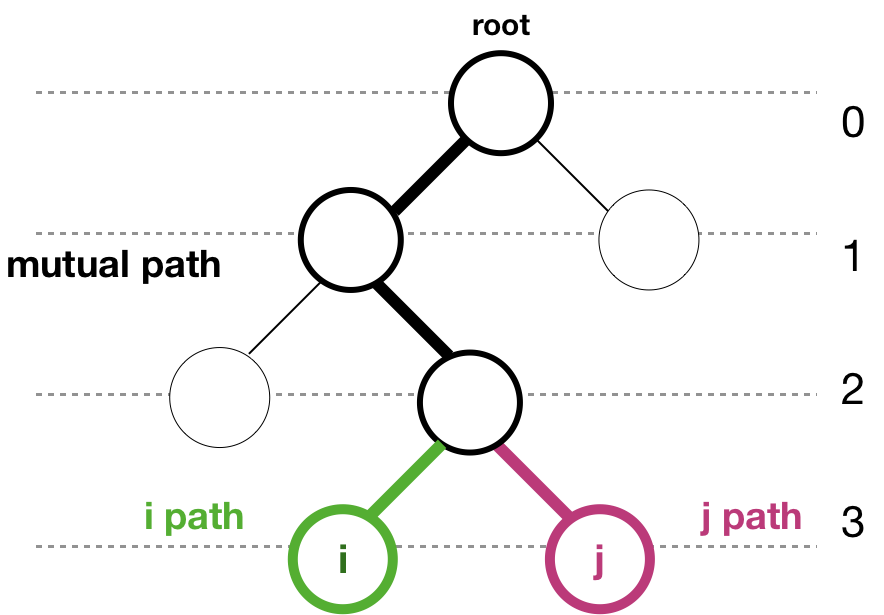
\includegraphics[height=0.5\textheight]{fig/ppath3.png}
    \end{figure}
  \end{frame}

  \begin{frame}{Implementation of modified RF}
    \begin{figure}
      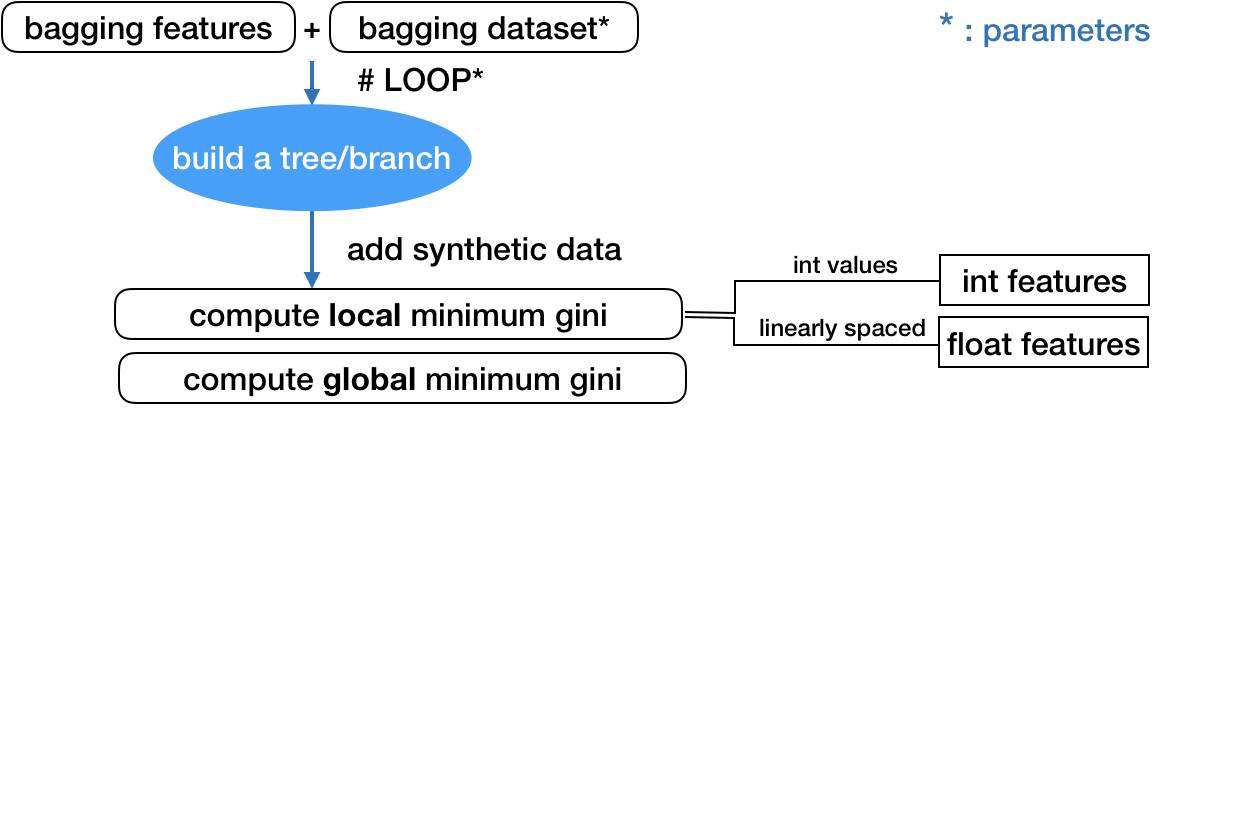
\includegraphics[height=0.8\textheight]{fig/decisiontree_diagram0.png}
    \end{figure}
    \end{frame}
  \begin{frame}{Implementation of modified RF}	
    \begin{figure}
      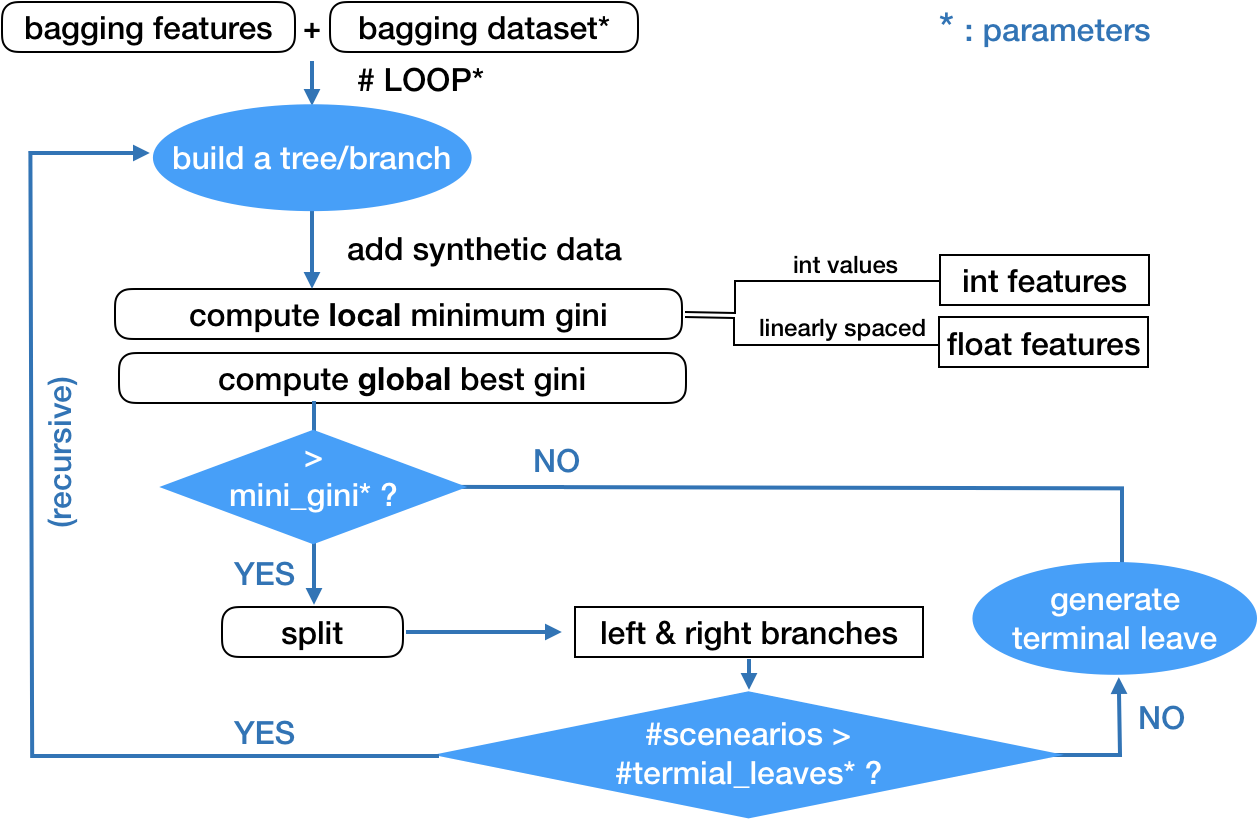
\includegraphics[height=0.8\textheight]{fig/decisiontree_diagram.png}
    \end{figure}
    \end{frame}

    \begin{frame}{Implementation of Proximity Matrix}	
      \begin{figure}
        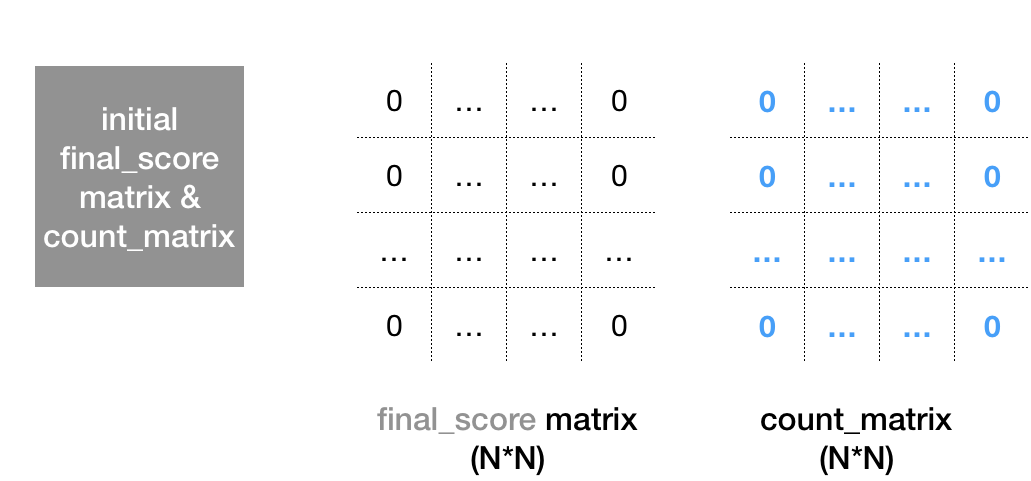
\includegraphics[height=0.6\textheight]{fig/proximity00.png}
      \end{figure}
    \end{frame}
    \begin{frame}{Implementation of Proximity Matrix}	
      \begin{figure}
        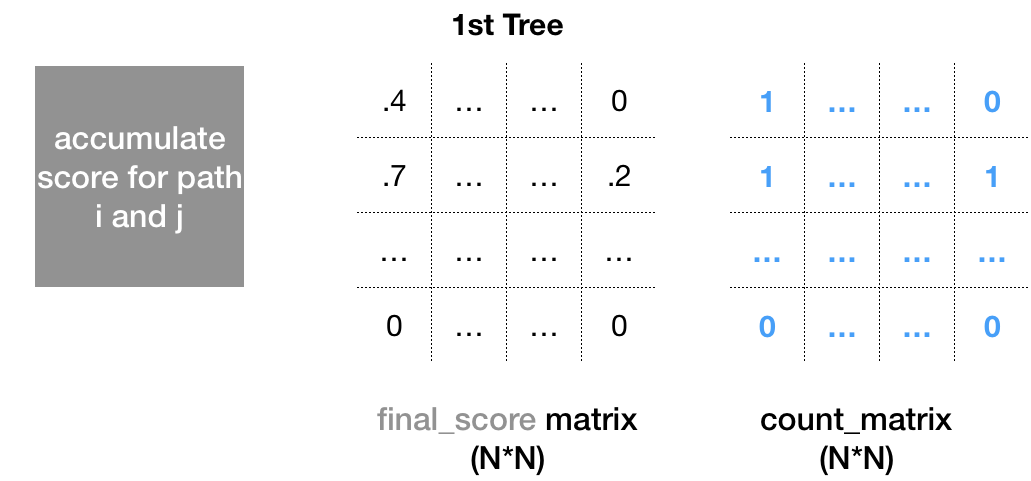
\includegraphics[height=0.6\textheight]{fig/proximity01.png}
      \end{figure}
    \end{frame}
    \begin{frame}{Implementation of Proximity Matrix}	
      \begin{figure}
        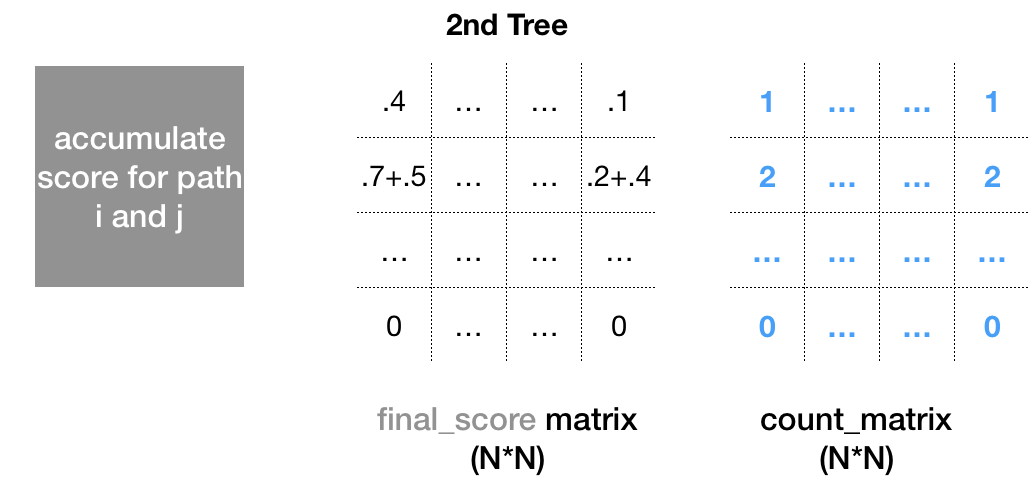
\includegraphics[height=0.6\textheight]{fig/proximity02.png}
      \end{figure}
    \end{frame}
    \begin{frame}{Implementation of Proximity Matrix}	
      \begin{figure}
        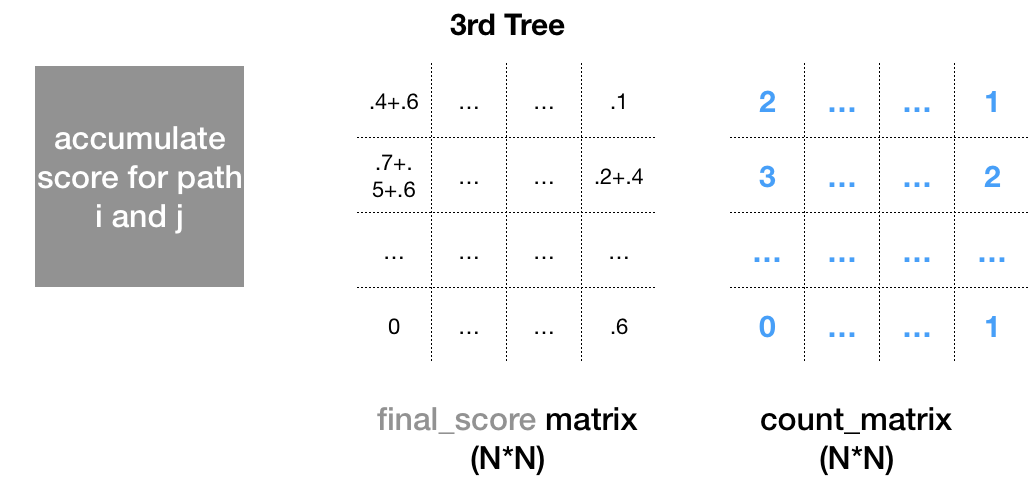
\includegraphics[height=0.6\textheight]{fig/proximity03.png}
      \end{figure}
    \end{frame}
    \begin{frame}{Implementation of Proximity Matrix}	
      \begin{figure}
        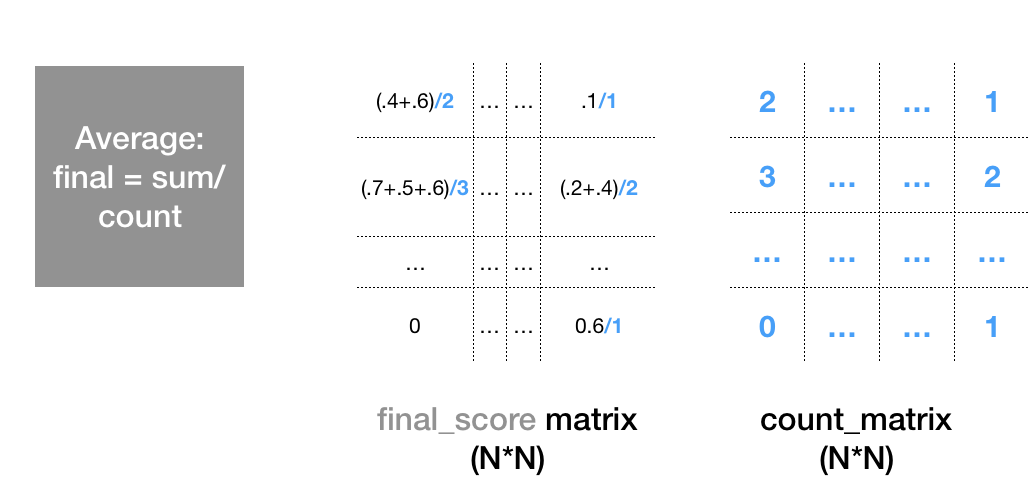
\includegraphics[height=0.6\textheight]{fig/proximity04.png}
      \end{figure}
    \end{frame}
    \begin{frame}{Implementation of Proximity Matrix}	
      \begin{figure}
        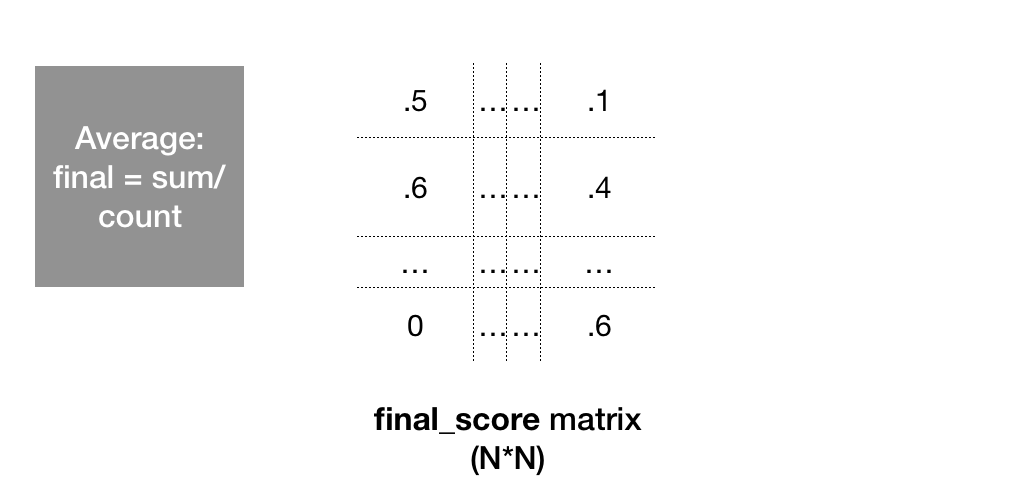
\includegraphics[height=0.6\textheight]{fig/proximity05.png}
      \end{figure}
    \end{frame}
    \begin{frame}{Implementation of Proximity Matrix}	
      \begin{figure}
        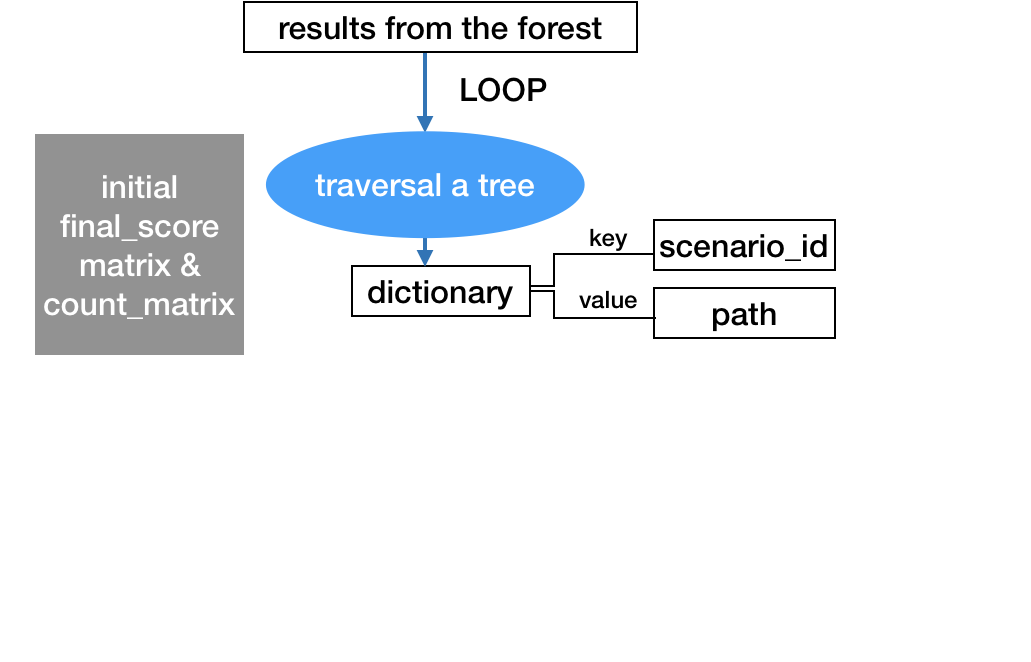
\includegraphics[height=0.8\textheight]{fig/proximity0.png}
      \end{figure}
    \end{frame}
   
    \begin{frame}{Implementation of Proximity Matrix}	
      \begin{figure}
        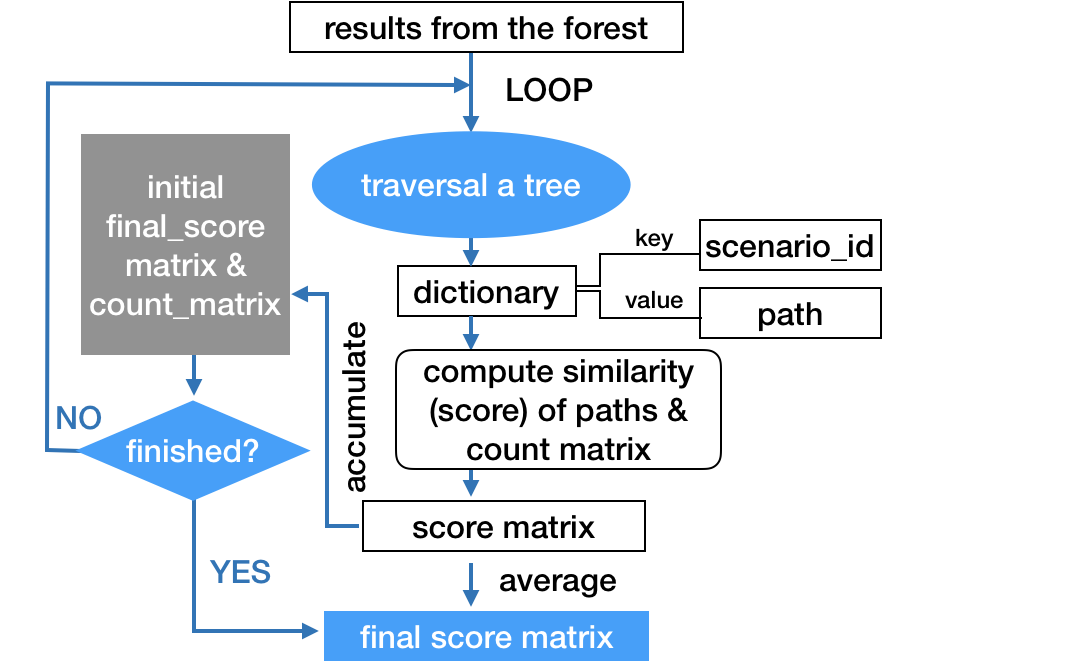
\includegraphics[height=0.8\textheight]{fig/proximity.png}
      \end{figure}
      \end{frame}
      \begin{frame}{From DataFrame to Proximity Matrix}	
        \begin{figure}
          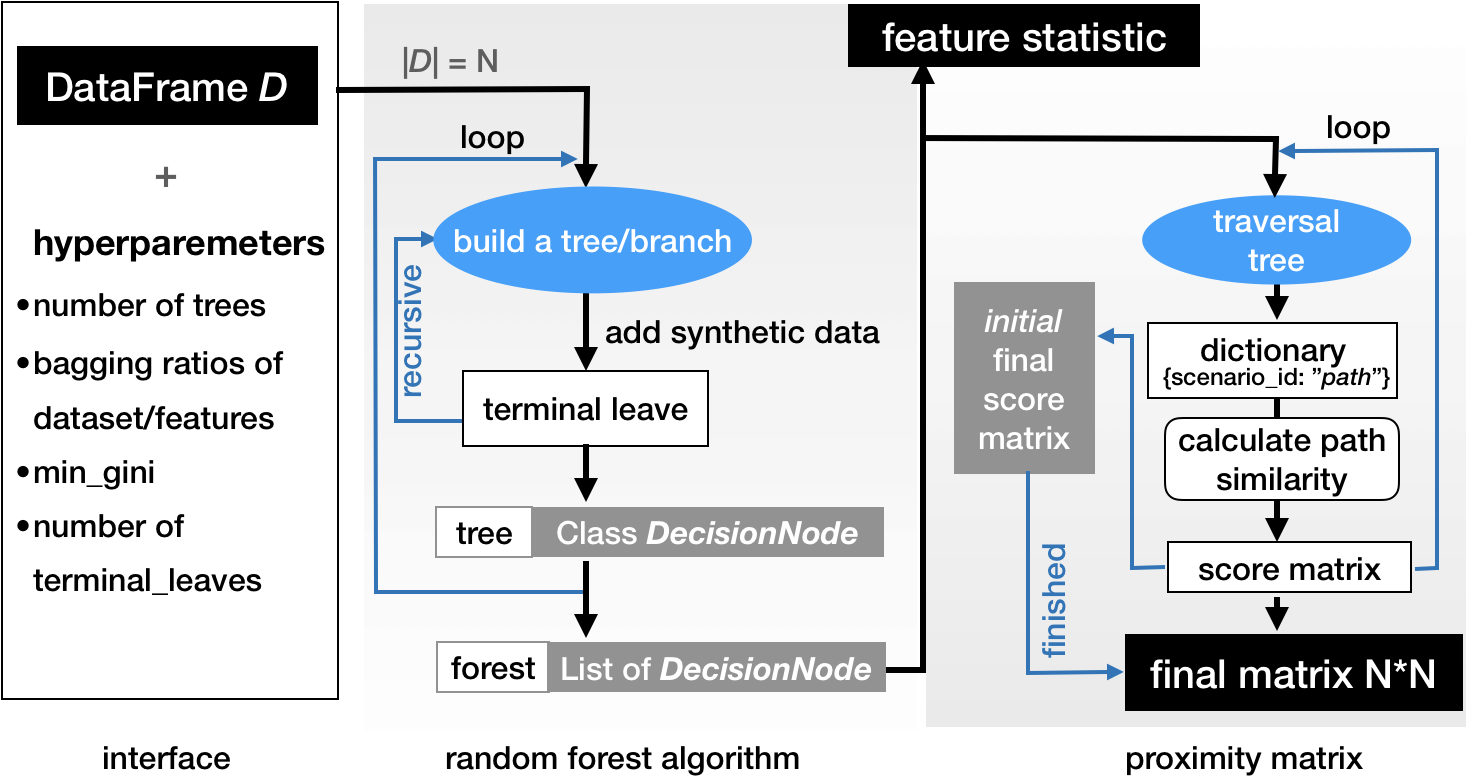
\includegraphics[height=0.74\textheight]{fig/dandp3.png}
        \end{figure}
        \end{frame}

\section{Clustering}

\begin{frame}{Improvements}
    \begin{itemize}
        \item Gini gain instead of gini index:
        $$ \Delta R(t, t_L, t_R)= r(t) - \frac{M(t_L)}{M(t)}r(t_L) - \frac{M(t_R)}{M(t)}r(t_R) $$
        \item Random distribution instead of equally spaced points
        \begin{itemize}
            \item Uniform
            \item Normal
            \item Bimodal (Gaussian mixture)
        \end{itemize}
        \item Variable proportion of synthetic points
    \end{itemize}
\end{frame}

\begin{frame}{Description}
    For each feature:
    \begin{enumerate}
        \item Transform the data to interval [-3, 3]
        \item Add synthetic points
        \item Find split with best gini gain
    \end{enumerate}
    Best feature determines number of synthetic points of children:
    \begin{equation}
    \begin{split}
        M_{S, l}(z) & = M_{D}(t) \textrm{Pr}(\textrm{Z} \leq z) \\
        M_{S, r}(z) & = M_{D}(t) - M_{S, l}(z)
    \end{split}
    \end{equation}
    Randomly choose a distribution for the children (add PDFs):
    $$ \textrm{Unif}(-3,3), \ \mathcal{N}(0,1) \textrm{ or } \mathcal{N}(-1,0.7^2) + \mathcal{N}(1,0.7^2) $$
\end{frame}

\begin{frame}{Trade-offs}
    \begin{center}
    \begin{tabular}{p{5cm}|p{5cm}}
        Advantages & Disadvantages \\
        \hline
        \hline
         Less dependent on distribution & Sensitive to distribution parameters \\
         \hline
         Continuous improvement & Deeper trees
    \end{tabular}
    \end{center}
    Problems encountered:
    \begin{itemize}
        \item Split contained no points to one side $\Rightarrow$ enforce borders, check spread
        \item Trees grew very deep $\Rightarrow$ clipping
        \item Similarity matrix has high values
    \end{itemize}
    	\vspace{+1em}
        \centering
        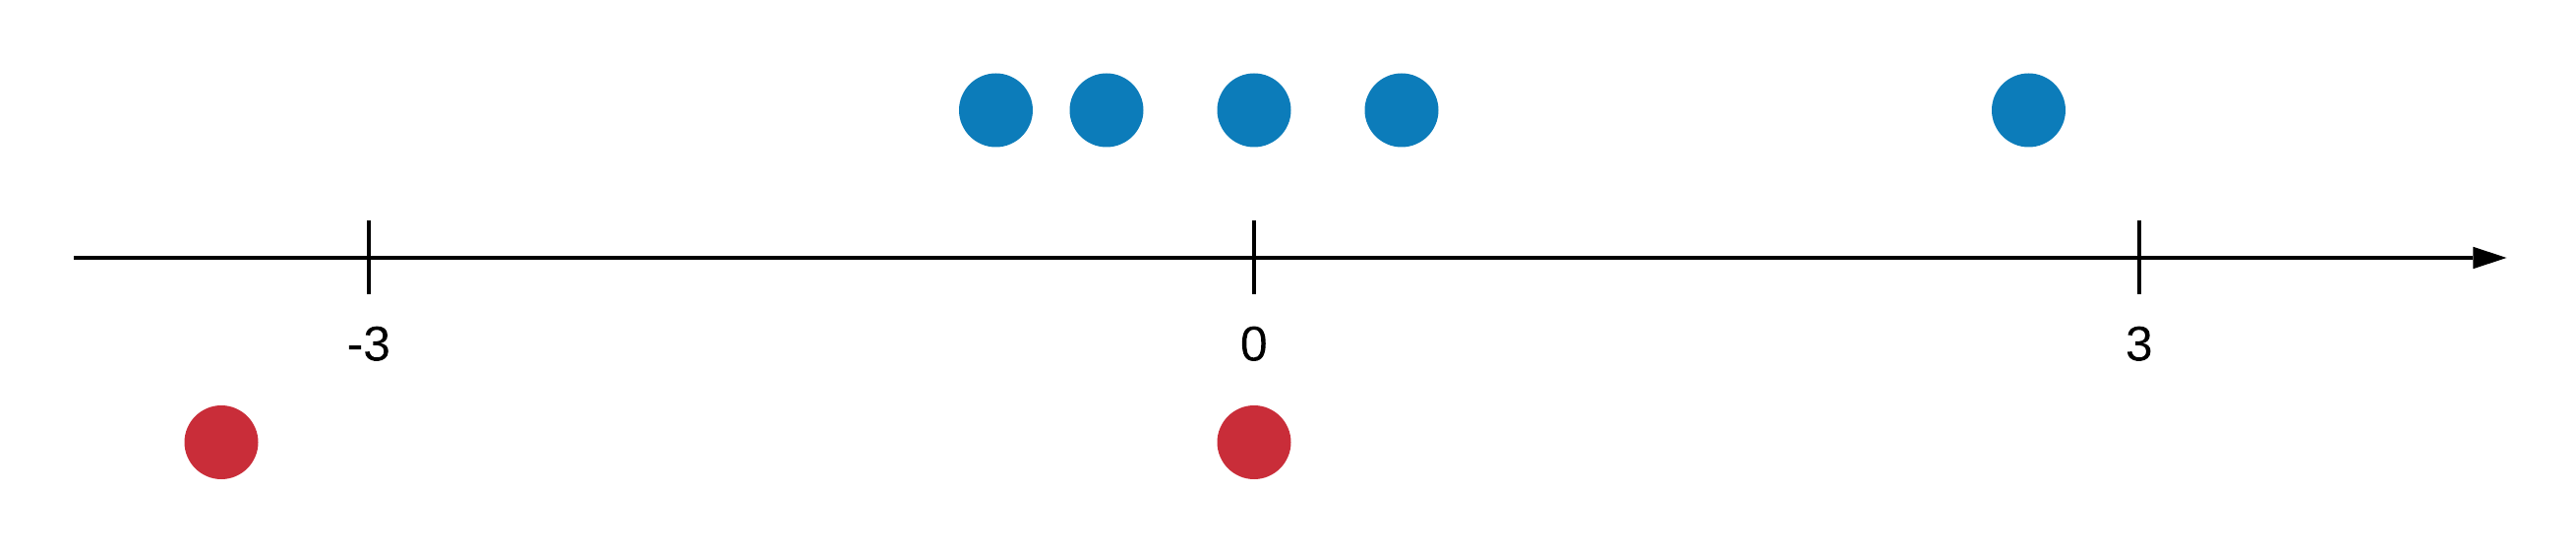
\includegraphics[width=\textwidth]{cut_off.png}
\end{frame}


\begin{frame}{Hierarchical Clustering}

\begin{columns}
\begin{column}{0.6\textwidth}
\begin{itemize}
\item \textbf{Goal:} Given a proximity matrix, compute clusters
\item \textbf{Procedure:} Sequentially group similar data points together
\item \textbf{Implementation:} CLI with most important parameters. Scikit-learn library
\item Questions:
\begin{itemize}
\item When to stop $\Rightarrow$ heat map, silhouette coefficient
\item How to compute distance between clusters $\Rightarrow$ try all
\end{itemize}
\end{itemize}
\end{column}
\begin{column}{0.4\textwidth}
\vspace{-1em}
\centering
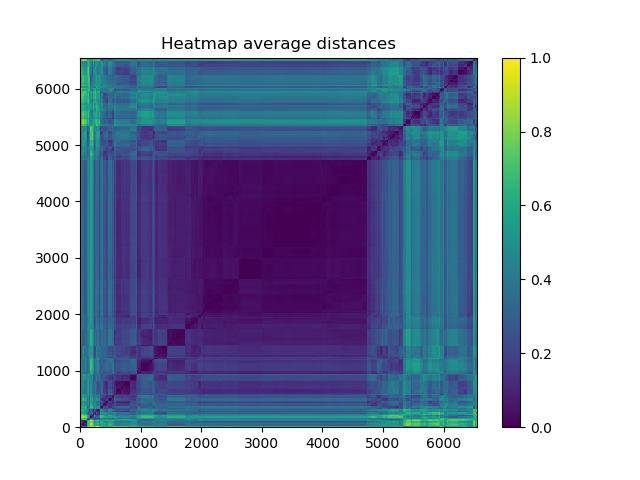
\includegraphics[width=\textwidth]{heatmap2.png}
\vspace{-2em}
\end{column}
\end{columns}

\end{frame}

\begin{frame}{Evaluation}
    \begin{columns}
    \begin{column}{0.6\textwidth}
    How to best evaluate our results?
    \begin{itemize}
        \item Dendrogram becomes unreadable at this size
        \item Heat map (cluster map)
        \item Boxplots (splitting, features)
        \item Animations
        \item Silhouette coefficient
    \end{itemize}
    \end{column}
    \begin{column}{0.4\textwidth}
        \centering
        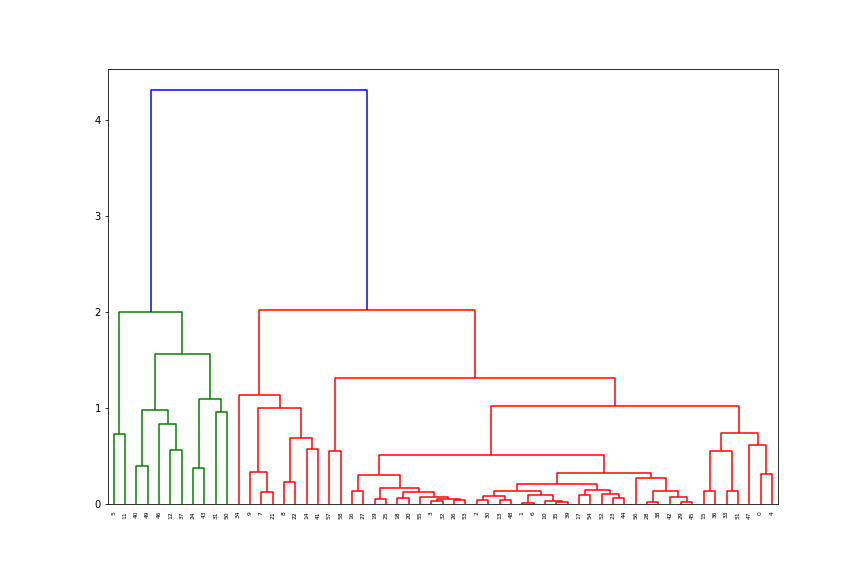
\includegraphics[width=\textwidth]{dendro.png}
    \end{column}
    \end{columns}
    
\end{frame}

\begin{frame}{One number}
Silhouette coefficient
    \begin{equation}
        \begin{split}
            a(i) & = \frac{1}{\lvert C_i \rvert} \sum_{j \in C_i, j \neq i} d(i, j) \\
            b(i) & = \min_{k \neq i}\frac{1}{\lvert C_k \rvert}\sum_{j \in C_k}d(i,j)\\
            s(i) & = \frac{b(i) - a(i)}{\max\{a(i), b(i)\}}, \textrm{ if } \lvert C_i \rvert > 1\\
            s(i) & = 1, \textrm{ if } \lvert C_i \rvert = 1
        \end{split}
    \end{equation}
$a(i)=$ average distance to points withing cluster \\
$b(i)=$ smallest average distance to another cluster \\
$s(i)$ close to $1 \Rightarrow$ good clustering, $-1 \Rightarrow$ overlaps \\
Generally better for convex clusters
\end{frame}

\begin{frame}{Splitting}
    \centering
    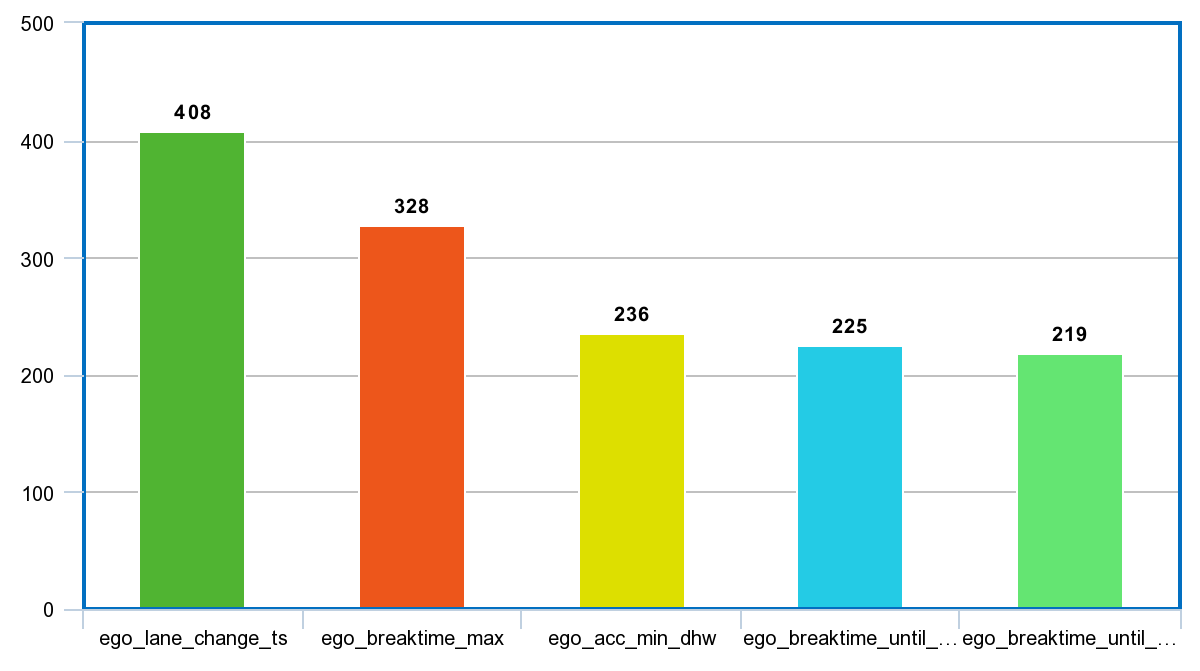
\includegraphics[width=\textwidth]{meta-chart.png}
    300 Trees with a total of 5718 splits
\end{frame}

\begin{frame}{Identifying the number of clusters}
    \begin{columns}
        \begin{column}{0.5\textwidth}
            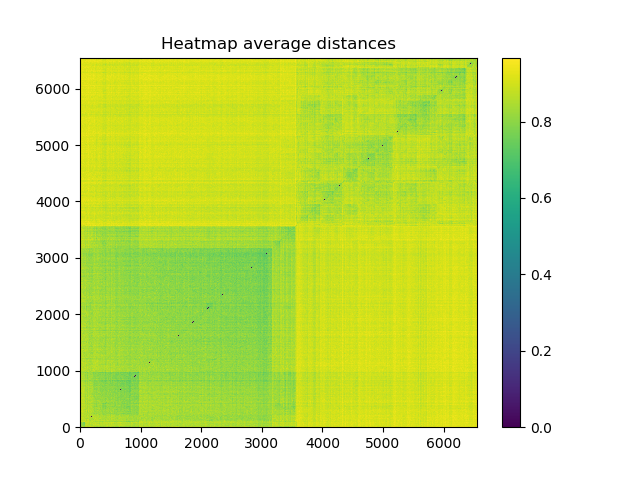
\includegraphics[width=\textwidth]{heatmap_average.png}
        \end{column}
        \begin{column}{0.5\textwidth}
            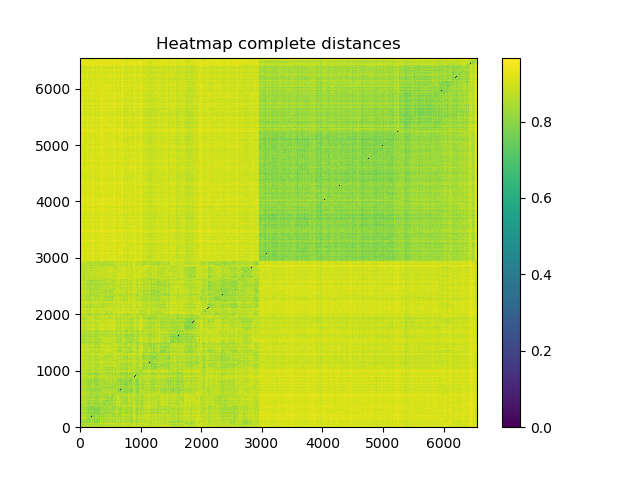
\includegraphics[width=\textwidth]{heatmap_complete.png}
        \end{column}
    \end{columns}
\end{frame}


\begin{frame}{Differences among clusters}

The two most used features on DHW dataset, 200 trees
{
\centering
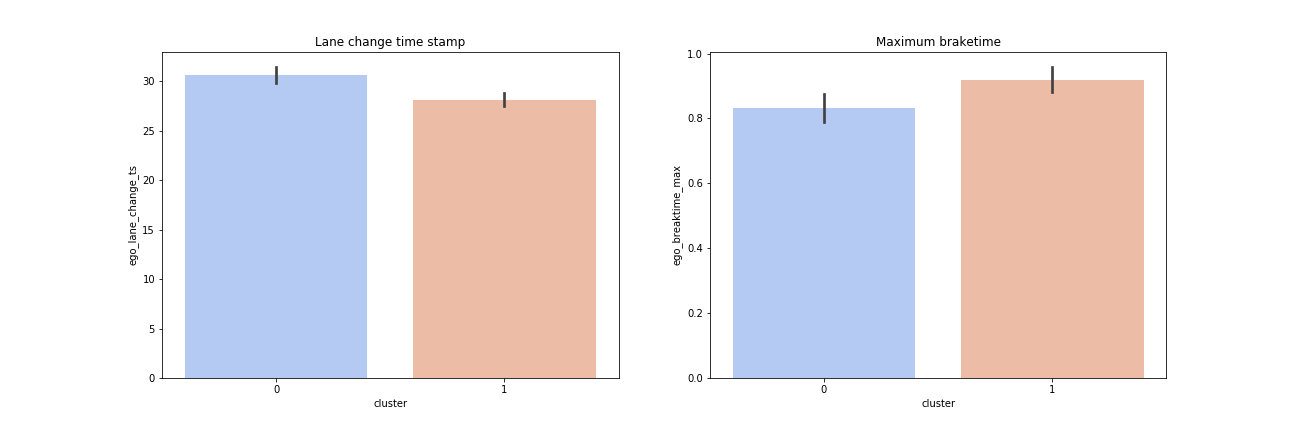
\includegraphics[width=\textwidth]{bar.png}
}
Differences are very small...

\end{frame}


\section{Conclusion}

\begin{frame}{Conclusion}

\begin{itemize} 
\item Data generation:
	\begin{itemize}
	\item Filtered out considerable amount of non-critical scenarios.
	\item Generated relatively more realistic scenarios based on sensor ranges.
	\end{itemize}
\item Clustering
\begin{itemize}
\item Higly sensitive to synthetic data
\item A lot of experiments needed
\end{itemize}
\end{itemize}

\end{frame}

\section{Future Work}

\begin{frame}{Future Work}

\begin{itemize} 
\item Data generation:
	\begin{itemize}
	\item Improve data generation part to have more balanced dataset.
	\item Further investigate edge cases during the scenario generation.
	\end{itemize}
\item Clustering:
	\begin{itemize}
        \item Adjust parameters and clean data
        \item Add a prediction part to the end of the pipeline
	\item Try different clustering approaches
    \end{itemize}
\end{itemize}

\end{frame}

\section{References}

\begin{frame}{References}
	\printbibliography
\end{frame}

\end{document}
